\PassOptionsToPackage{table}{xcolor}
\documentclass[]{article}


%\usepackage[table,xcdraw]{xcolor}
\usepackage{booktabs}
\usepackage{setspace}
\usepackage{amsmath}
\usepackage{amssymb}
\usepackage{graphicx}
\usepackage[a4paper,top=2cm,bottom=3cm,left=4cm,right=4cm]{geometry}
\usepackage{caption}
\usepackage[svgnames]{xcolor}
\usepackage{listings}
\usepackage{float}
\usepackage[T1]{fontenc}

\lstset{language=R,
	basicstyle=\small\ttfamily,
	stringstyle=\color{DarkGreen},
	otherkeywords={0,1,2,3,4,5,6,7,8,9},
	morekeywords={TRUE,FALSE},
	deletekeywords={data,frame,length,as,character},
	keywordstyle=\color{blue},
	commentstyle=\color{DarkGreen},
}

\usepackage{subfigure}
\usepackage{lipsum}
\usepackage[utf8]{inputenc}

\newenvironment{rcases}
{\left.\begin{aligned}}
	{\end{aligned}\right\rbrace}

\usepackage{hyperref}
\hypersetup{
	colorlinks,
	citecolor=black,
	filecolor=black,
	linkcolor=black,
	urlcolor=black
}

\makeatletter
\setlength{\@fptop}{0pt}
\makeatother

\DeclareMathOperator{\E}{\mathbb{E}}
\renewcommand{\figurename}{Figura}
\renewcommand{\tablename}{Tabella}




\renewcommand{\baselinestretch}{1.5} 
\renewcommand{\contentsname}{Indice}
\renewcommand{\listfigurename}{Elenco delle figure}
\renewcommand{\listtablename}{Elenco Tabelle}
\renewcommand\refname{Bibliografia}





\begin{document}


\tableofcontents
\break
\listoffigures
\cleardoublepage

\newpage 


\topskip0pt
\vspace*{6cm}
	\begin{flushright}
	\textit{A Mamma,\\ non temo alcun male perchè tu sei con me.}
\end{flushright}
\vspace*{\fill}

%\



\newpage

%%%%%%%%%%%%%%%
% INTRODUZIONE
%%%%%%%%%%%%%


\section*{Introduzione}
\addcontentsline{toc}{section}{Introduzione}

Questo lavoro ha l’obiettivo di sviluppare e analizzare una strategia di investimento finanziario mediante strumenti econometrici. 
L'utilizzo di alcuni principi dell'econometria finanziaria nel mondo del \textit{trading} ha, negli anni, assunto un ruolo sempre più preponderante. La necessità di sviluppare strategie di investimento sempre più complesse, connesse con il rapido sviluppo tecnologico del mondo finanziario e la rapida ascesa dei sistemi automatizzati di trading, ha portato alla nascita di differenti strategie operative che sfruttano modelli matematici e statistici al fine di competere con il mercato.
In questo lavoro tratteremo, dal punto di vista matematico e statistico, alcuni dei concetti econometrici ampiamente utilizzati nel mondo della finanza. Più specificatamente, oggetto di questa tesi, sarà lo sviluppo di un modello operativo basato su una strategia di arbitraggio statistico definita \textit{pair trading} o trading di coppia.
L'idea generale dietro la costruzione di una strategia di pair trading è quella di sfruttare, basandosi su un analisi relativa dei prezzi, il \textit{mispricing} di due assets cointegrati, vendendo il relativo asset sopravvalutato e acquistando l'asset sottovalutato.
In questa tipologia di analisi il prezzo specifico del titolo assume una importanza relativa, ciò che conta è la relazione che lega i prezzi dei due titoli. In questo senso il pair trading fonda la sua operatività sulla generazione di segnali opposti. In particolare viene assunta una posizione lunga sul titolo che ha un prezzo troppo basso ed una posizione corta su quello che ha un prezzo troppo elevato, nell’attesa che il mispricing si corregga.
Nel corso di questo lavoro saranno trattate dettagliatamente tutte le fasi che hanno portato alla costruzione del modello operativo e all'implementazione della strategia di trading connessa.
Nei Capitoli 1,2 e 3 vengono presentati gli strumenti matematici e statistici che sono indispensabili per affrontare le diverse metodologie che saranno sviluppate nel corso del lavoro. Vengono formalizzati i concetti di cointegrazione e serie storiche cointegrate, i modelli lineari nello stato degli spazi e l'applicazione di un Kalman Filter.
\\
L’ultima sezione descrive la concreta applicazione del modello operativo. In quest’ultima parte la trattazione è sviluppata mediante un duplice approccio. Da un lato si considera la gestione del portafoglio. Tramite il Back Testing della strategia infatti, vengono rilevati i risultati in termini di rischi e rendimento. Questa analisi è effettuata mediante le tecniche di valutazione delle performance e del rischio tipiche dell'asset allocation. A questa segue lo studio del modello e la valutazione dei suoi risultati da un punto di vista econometrico. Da ultimo l’Appendice teorica sintetizza la teoria econometrica utilizzata nelle applicazioni pratiche sviluppate.
La costruzione ed il Back Testing della strategia, con particolare riferimento ai test econometrici, vengono implementati mediante l’utilizzo del software statistico R (www.r-project.org). Tale linguaggio di programmazione è stato scelto per la duttilità e per la sua caratteristica di essere liberamente disponibile ed open-source. Questo fa si che i risultati di un lavoro di ricerca sviluppato in R siano verificabili da chiunque intenda effettuare un controllo per dare una valutazione del lavoro.
A tale scopo sono riportati in Appendice gli script della programmazione utilizzata nella costruzione del modello.

\break 

\section{Statistical Arbitrage}

In finanza, l'arbitraggio statistico (spesso abbreviato in Stat Arb o StatArb ) è una classe di strategie di trading finanziario a breve termine che impiegano modelli di ritorno alla media.
In generale, si creano opportunità di arbitraggio statistico quando si riescono ad individuare delle componenti sistematiche nelle dinamiche dei prezzi di alcuni asset che si muovono con regolarità persistenti e prevalenti, e dunque per gli arbitraggisti  è facile prevedere l’andamento di tali prezzi e sviluppare strategie di trading per speculare. 
Il primo utilizzo di una strategia di trading a coppie è attribuito al \textit{quant} di Wall Street Nunzio Tartaglia, che era alla Morgan Stanley a metà degli anni '80.
Sebbene esistano strategie di arbitraggio statistico molto complesse,il concetto base dietro una strategia di pair trading è piuttosto semplice.
\\
Informalmente parlando, se due titoli hanno caratteristiche simili, i prezzi di entrambi gli asset devono essere più o meno gli stessi; cioè, mantengono un certo grado di equilibrio. Se i prezzi divergono, è probabile che uno degli asset sia troppo caro e/o l'altro sia sottovalutato. Fondamentalmente, strategie di pair trading comportano la vendita dell'attività a prezzo più alto e l'acquisto dell'attività a prezzo più basso con la speranza che l'errata valutazione venga infine corretta dal valore di equilibrio a lungo termine. Pertanto, l'idea alla base di una determinata strategia di pair trading è di operare sulle oscillazioni attorno al valore di equilibrio dello spread. Le oscillazioni dello spread si verificano perché quest'ultimo è presumibilmente mean-reverting. Si può aprire un'operazione quando lo spread si discosta sostanzialmente dal suo valore di equilibrio e chiudere l'operazione quando l'equilibrio viene ripristinato. Affinché l'operazione sia redditizia, la deviazione deve essere ragionevolmente maggiore dei costi di negoziazione.
La peculiarità del \textit{pair trading} è la sua neutralità rispetto al mercato.Pertanto, questa strategia si sforza di fornire rendimenti positivi sia nei mercati rialzisti che ribassisti selezionando un gran numero di posizioni lunghe e corte senza esposizione netta al mercato. 
Sebbene rientri nelle cossiddette \textit{market neutral strategies},
tuttavia, le strategie di pair trading non sono del tutto vero arbitraggio statistico, nel senso che si basano sulla prevedibilità congiunta degli asset e quindi non sono esenti da rischi.
I principali rischi insiti in una negoziazione di coppie sono i seguenti: 
\begin{enumerate}
	\item Rischio di divergenza: la relazione di equilibrio a lungo termine tra le attività può cambiare o addirittura svanire; 
	\item Rischio di orizzonte: lo spread non converge in un dato orizzonte di tempo, costringendo quindi i traders a chiudere la posizione prima della convergenza, a causa di un peggioramento dei prezzi o delle richieste di margine 
\end{enumerate}
La letteratura accademica può essere suddivisa in due approcci principali, sebbene Huck, Afawubo (2015) e Krauss (2017) potrebbero argomentare diversamente.
Il primo approccio  la distanza minima al quadrato (SSD), essendo uno dei primi approcci da implementare. Segue, la cointegrazione. Per questo studio utilizzeremo l'approccio della cointegrazione e non ci soffermeremo sugli altri possibili approcci. Insieme alla letteratura recente, in questo studio ci poniamo anche la domanda se il trading di coppi sia una strategia ancora redditizia. Inoltre, questo studio differisce da altra letteratura, in diversi aspetti. Analizzeremo  le prestazioni di un strategia di Pairs trading con modelli diversi; il normale approccio cointegrato, una stima "rolling" della cointegrazione conuna finestra bimestrale e un approccio di stima dinamica gionaliera della cointegrazione, attraverso l'utilizzo di un Kalman Filter.

\break 

\section{Cointegrazione}

\subsection{Serie storiche cointegrate}
La definizione di cointegrazione è dovuta all’econometrico C.W.J. Granger che per tale ricerca è stato insignito, insieme a R.F. Engle, del premio Nobel per l’economia nel 2003.
\\
Per introdurre la cointegrazione tra due serie temporali è utile definire il concetto di integrazione di una serie storica.
\\
Una serie temporale $x_t$ è definita integrata di ordine 1, $I(1)$, se non è stazionaria, ma è stazionaria nelle prime differenze $\Delta x_t= x_t - x_{t-1}$.
\\
Il concetto di cointegrazione prende invece in esame due serie temporali: \\ due serie temporali $y_t$ e $x_t$, integrate di ordine $I(1)$, sono cointegrate se la loro combinazione lineare è un processo debolmente stazionario, I(0).
\\
In altre parole il concetto di cointegrazione prende in esame la relazione tra due variabili, $y_t$ e $x_t$,
\begin{equation} 
	\hat{\epsilon} = y_t - \hat{\beta}x_t - \hat{\alpha}
\end{equation}
\\
in cui la presenza del vettore di cointegrazione, $\hat{\beta}$ ,rende possibile l'esistenza di un processo,$\epsilon_t$, lineare stazionario.
Generalmente l'approccio per testare se la combinazione di due serie storiche integrate produce un processo stazionario è quella di stimare dapprima i parametri $\alpha$ e $\beta$ attraverso una regressione lineare, dopodichè testare la presenza di una radice unitaria all'interno del processo $\epsilon_t$. Questo approccio definito anche \textbf{Engle-Granger two-step method} prevede l'utilizzo di una particolare statistica test denominata \textbf{ADF-Test}, ampiamente e più formalmente trattata nell'Appendice teorica.
In termini meno formali, il concetto di cointegrazione tra due variabili esprime la presenza di una relazione di lungo equilibrio statico nel tempo. Questo si verifica quando due serie temporali che si comportano come random walk (processi non stazionari, come nel caso dei prezzi azionari), sebbene siano tra di loro e individualmente processi casuali, sono in qualche modo legati da un \textit{trend} comune, almeno nel lungo periodo. Ciò ci consente, con ragionevole dubbio, di conoscere la posizione di una variabile dalla posizione della sua cointegrante.

\break
\section{Linear State Space Models}

\begin{figure}[!htp]
	\begin{center}
		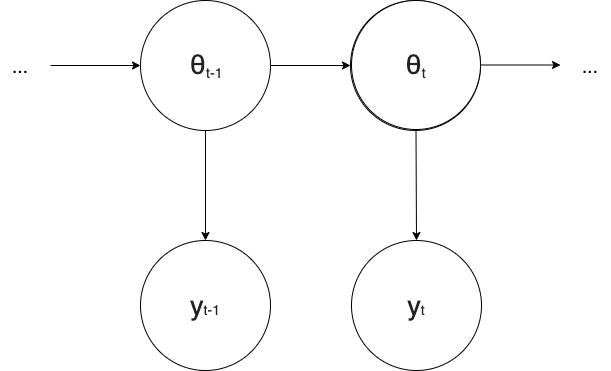
\includegraphics[scale=0.3]{download.png}
		\caption{\textbf{Diagramma di uno State space model}}
	\end{center}
\end{figure}
\
\\
Gli State Space Models (Modelli nello Spazio degli Stati) forniscono una metodologia generale di riferimento, molto flessibile, per affrontare una vasta gamma di problemi nell’analisi delle serie storiche.
L’idea metodologica alla base degli State Space Models è che lo
sviluppo nel tempo del fenomeno in analisi, $y_1....y_n$ , sia determinato da una serie di vettori non osservabili $\theta_1....\theta_n$.
\\
La relazione tra $y_t$ e $\theta_t$ specifica il modello nella forma state space.



\subsubsection{Time-varying coefficients}
La relazione lineare tra due variabili cointegrate è descritta da:
\begin{equation}\label{classic_cointegration}
	y_t = \alpha + \beta x_t + \epsilon_t
\end{equation}
\\
In cui $\alpha$ e $\beta$ sono invarianti nel tempo.
La formulazione dell'equazione \ref{classic_cointegration} come un modello state space Gaussiano ci permette di considerare invece l'evoluzione degli stati $\alpha$ e $\beta$ nel tempo. Assumendo che questi si evolvano secondo un processo random walk avremo che \footnote{J. Durbin and S. J. Koopman, Time Series Analysis by State Space Methods, 2nd Ed. Oxford University Press, 2012}:
\begin{align}
	y_t = \alpha_t + \beta_t x_t + \epsilon_t\\
	\alpha_t = \alpha_{t-1} + \eta_{1,t}\\        
	\beta_t = \beta_{t-1} + \eta_{2,t}
\end{align}
\\
Il modello state space gaussiano è quindi definito da due equazioni\footnote{Daniel P. Palomar- Portfolio Optimization with R - The Hong Kong University of Science and Technology (HKUST)}:
\begin{align}
		\theta_{t}=T_t\theta_{t-1} + \eta_t\\   
		y_t = Z_t\theta_t + \epsilon_t 
\end{align}
\
\begin{itemize}
	\item $\theta_t \triangleq \begin{bmatrix}
		\alpha_t\\
		\beta_t
	\end{bmatrix}$ è lo stato inosservato
	
	\item $T_t \triangleq \begin{bmatrix}
		1 & 0 \\
		0 & 1
	\end{bmatrix}$ è la matrice di transizione degli stati
	
	\item $\eta_t \sim \mathcal{N}(0,Q)$ è detto \textbf{state transition noise} ed è un errore gaussiano a media 0 e con matrice di covarianza $Q \triangleq \begin{bmatrix}
		\sigma^2_1 & 0 \\
		0 & 	\sigma^2_2
	\end{bmatrix}$
	
	\item $Z_t \triangleq  \begin{bmatrix}
		1 & x_t
	\end{bmatrix}$ è la matrice di osservazione, dove $x_t$ rappresenta,nel nostro caso,un vettore di prezzi.
	
	\item $\epsilon_t \sim \mathcal{N}(0,\sigma^2_e)$ è detto \textbf{observation noise} 
\end{itemize}
\
\\
L'eq. 6 è definita \textbf{equazione di transizione} ed esprime la transizione dello stato $\theta_t$ attraverso una relazione lineare.
\\
L'eq. 7 è invece definita \textbf{equazione di misurazione} ed esprime la relazione lineare tra lo stato di osservazioni $y_t$ e lo stato latente $\theta_t$.
\\
Una volta specificato il modello in forma state space, la stima degli stati inosservati $\theta$ può essere ottenuta in maniera ricorsiva attraverso l'utilizzo di un Kalman Filter.
\\

\subsubsection{Filtro ricorsivo}
L’obiettivo nell’applicazione del Kalman Filter è l’aggiornamento
della conoscenza (cioè, informazioni) del fenomeno oggetto di studio
ogni volta che una nuova osservazione è aggiunta alla serie storica.
Considerato che tutte le distribuzioni sono normali, anche le
distribuzioni congiunte condizionate di un insieme di osservazioni
dato un altro insieme di osservazioni sono normali.
\\
Indichiamo $Y_{t-1} = {y_1,...,y_{t-1}}$ e assumiamo che la distribuzione condizionata di $\theta_t$ dato $Y_{t-1}$ sia normale,cioè $Pr(\theta_t|Y_{t-1})= \mathcal{N}(a_t,P_t)$.
\
L'obiettivo è calcolare $a_{t+1}$ e $P_{t+1}$ quando l'osservazione $y_t$ è aggiunta alla serie storica.
Definiamo quindi
\begin{align}
	a_{t+1} = \E(\theta_{t+1}|Y_t) = \E(\theta_t + \eta_t| Y_t) = \E(\theta_t|Y_t) 
	\\
	P_{t+1} = Var(\theta_{t+1}|Y_t) = Var(\theta_t|Y_t) + \sigma_{\eta}^2
\end{align}
\
La previsione dell'errore chiamata  $\mathbf{v_t}$ è definita come
\begin{equation}
	\begin{split}
		v_t & = y_t - \E(y_t|Y_{t-1})    \\
		& = y_t - \E(\theta_t|Y_{t-1}) \\
		& = y_t - a_t
	\end{split}
\end{equation}
\
e indichiamo con $\mathbf{F_t= Var(v_t)= P_t + \sigma_{\epsilon}^2}$ la sua varianza.
\\
Il modello lineare nello stato degli spazi è poi ricorsivamente aggiornato per $t=1,...,n$ 
\begin{gather*}
	 K_t = \frac{P_t}{F_t}
	 \\
	 a_{t+1} = a_t + K_tv_t
	 \\
	 P_t = K_t\sigma_{\epsilon}^2
	 \\
	 P_{t+1} = P_t + \sigma_{\eta}^2
\end{gather*}

\subsubsection{Una formulazione Bayesiana}

Il termine Kalman Filter o Kalman Filtering fa riferimento ad una procedura ricorsiva che permette di conoscere la vera natura dello stato $\theta_t$. La nozione chiave è che possiamo fare inferenza su $\theta_t$ attraverso una diretta applicazione del teorema di Bayes, in altre parole 
\begin{equation}
	Pr(Natura \; dello \; stato| Dati) \propto Pr(Dati| Natura\; dello \; stato)
\end{equation}
\
che può essere scritto come 

\begin{equation}
	P(\theta_t|Y_t) \propto P(Y_t| \theta_t,Y_{t-1}) \cdot P(\theta_t|Y_{t-1})
	\label{dist_post}
\end{equation}
\
dove i due termini alla destra dell'equazione sono rispettivamente la verosimiglianza e la distribuzione a priori dello stato latente. Il termine sulla sinistra è la distribuzione a posteriori dello stato $\theta$.
\\
L'inizializzazione del filtro ricorsivo parte dall'assunzione (o dalla stima) dei parametri che definiscono la distribuzione dello stato $\theta$. Nella sezione successiva è stato trattato nel dettaglio l'utilizzo dei parametri necessari per l'inizializzazione della procedura ricorsiva.
Al fine di spiegare al meglio i passaggi, inizieremo considerando lo stato del sistema al tempo t-1.
Al tempo t-1, la nostra conoscenza dello stato $\theta_{t-1}$ è rappresentato dalla seguente distribuzione di probabilità
\begin{equation}
	(\theta_{t-1}|Y_{t-1}) \sim \mathcal{N}(\hat{\theta}_{t-1},\Sigma_{t-1})
	\label{theta_meno1}
\end{equation} 
\
dove $\hat{\theta}_{t-1}$ e $\Sigma_{t-1}$ sono il valore atteso e la varianza della distribuzione a posteriori di $\theta_{t-1}$.
Sottolineiamo come anche nella formulazione bayesiana del filtro ricorsivo, parliamo di un modello nello spazio degli stati di matrice Gaussiana.
\\
Prima di osservare $Y_t$ la nostra miglior scelta per $\theta_t$ è rappresentata da

\begin{equation}
	\theta_t = T_t \theta_{t-1} + \eta_t
\end{equation}
siccome $\theta_{t-1}$ è descritta dall'eq. \ref{theta_meno1} la nostra conoscenza dello stato $\theta_t$ è rappresentata da

\begin{equation}
	(\theta_t|Y_{t-1}) \sim \mathcal{N}(T_t \hat{\theta}_{t-1}, T_t  \Sigma_{t-1} T_t' + \eta_t)
\end{equation}
\
che è la nostra distribuzione a priori normale.
\\
Definiamo $v_t $ l'errore di previsione o meglio
\begin{equation}
	v_t = Y_t - \hat{Y_t} = Y_t - T_t Z_t \hat{\theta}_{t-1}
\end{equation}
\
siccome ii parametri $Z_t$ e $T_t$ sono specificati osservare $Y_t$ equivale a dire che stiamo osservando $v_t$.
\\
In termini più formali avremo che 
\begin{equation}
	P(\theta_t|Y_t,Y_{t-1}) = P(\theta_t|v_t,Y_{t-1}) \propto P(v_t| \theta_t,Y_{t-1}) \cdot P(\theta_t|Y_{t-1})
\end{equation}
\
grazie all'eq. 7 possiamo scrivere che

\begin{equation}
	v_t = Z_t(\theta_t - T_t \hat{\theta}_{t-1}) 
\end{equation}
\
per cui 

\begin{equation}
	\E(v_t|\theta_t,Y_{t-1}) = Z_t(\theta_t - T_t \hat{\theta}_{t-1}) 
\end{equation}
\
Siccome  $\epsilon_t \sim \mathcal{N}(0,\sigma^2_e)$ la verosimiglianza è descritta da
\begin{equation}
	(v_t | \theta_t,Y_{t-1}) \sim \mathcal{N}( Z_t(\theta_t - T_t \hat{\theta}_{t-1}) , \sigma^2_e)
\end{equation}
\
Dal teorema di Bayes otteniamo 

\begin{equation}
	P(\theta_t|Y_t,Y_{t-1}) = \frac{P(v_t|\theta_t,Y_{t-1})\cdot P(\theta_t| Y_{t-1})}{\int P(v_t,\theta_t| Y_{t-1} d\theta_t}
	\label{final}
\end{equation}
\
che a meno di costanti di proporzionalità è la stima a posteriori dell'eq. \ref{dist_post}, coniugata a priori con una normale. 
L'eq. \ref{final} descrive la nostra conoscenza dello stato $\theta$ al tempo t.
\\
Una volta ottenuta la stima a posteriori di $\theta_t$ il filtro ricorsivo ricomincia dall'eq. \ref{theta_meno1}.


\subsubsection{Inizializzazione del Kalman Filter}
Il Kalman Filter per il modello gaussiano definito dalle equazioni (6) e (7)
viene inizializzato con l'ipotesi base
\begin{equation}
	\theta_0 \sim \mathcal{N}(\theta_0,\Sigma_0)
\end{equation}
\
in cui
\begin{itemize}
	\item $\theta_0 \triangleq \begin{bmatrix}
		\alpha\\
		\beta
	\end{bmatrix}$ coincidono con le stime dei parametri ottenuti del \textit{formation period}
	\item $\Sigma_0 \triangleq \begin{bmatrix}
		0.0001 & 0 \\
		0 & 0.0001
	\end{bmatrix}$ questo specifica che le varianze responsabili dell'incertezza \\\\
 attorno al parametro $\theta$ sono assunte di ordine molto piccolo, prossimo allo zero.
\end{itemize}
\


%%%%%%%%%%%
% ANALISI SPERIMENTALE
%%%%%%%%%%%

\break

\section{Pair trading}

\subsection{Individuazione del periodo di operatività}

L'analisi empirica è stata svolta considerando i prezzi di chiusura giornalieri, aggiustati per i dividendi, dei costituenti dell'indice FTSE MiB nel periodo dal 1° gennaio 2015 al 31 dicembre 2019.\footnote{I prezzi di chiusura giornalieri, aggiustati per i dividendi, sono stati ottenuti tramite Yahoo Finance}
\\
Il campione ottenuto è stato poi diviso in:

\begin{itemize}
	\item \textbf{\textit{Formation Period}}: Dal 1° gennaio 2015 al 31 dicembre 2018 (4 anni)
	\item \textbf{\textit{Trading Period}}::  Dal 1° gennaio 2019 al 31 dicembre 2019 (1 anno)
\end{itemize}
\
\\
Il \textit{Formation Period}(periodo di \textit{formazione}) è la fase di analisi delle serie storiche in cui vengono raccolte le informazioni alla base del \textit{trading} attuato nella fase successiva.
Nel \textit{Trading period}(periodo di \textit{trading}), formato dai 252 giorni di quotazione successivi al \textit{formation period} la strategia viene applicata sul mercato, costituendo di fatto la fase operativo dello studio.


\subsection{Analisi della relazione di cointegrazione}

Nel \textit{formation period}, per i 40 titoli dell'indice è stata analizzata la relazione di cointegrazione tramite l'Engle-Granger two-step method.
Da un punto di vista pratico sono state calcolate quindi $\frac{n^2-n}{2}$ possibili combinazioni di titoli tra i 40 presi in oggetto, per un totale di 561 combinazioni.
Per ognuna di queste combinazioni 
sono stati stimati i parametri $\hat{\alpha}$ e $\hat{\beta}$ attraverso una regressione lineare, per poi testare la stazionarietà o presenza di una radice unitaria nella combinazione lineare tra due titoli.

\subsection{Selezione delle coppie cointegrate}

Stimata la relazione di cointegrazione per le 561 combinazioni di titoli è stato scelto di selezionare le coppie che presentavano specifiche caratteristiche, ritenute ideali per l'implementazione della strategia di \textit{pair trading}.
La prima selezione è stata effettuata partendo da considerazioni sulle statistiche test individuate.
Sono state selezionate quindi quelle coppie la cui combinazione lineare nel \textit{formation period} generava un processo stazionario, per fare ciò sono ci siamo basati sull'ADF test.
Più specificatamente sono state scelte le combinazioni di titoli che permettevano di rifiutare l'ipotesi nulla di \textit{non stazionarietà} del processo ad un livello di confidenza del  5\%.
Una seconda selezione è stata effettuata tenendo conto del settore in cui opera un titolo quotato in borsa.
Se la relazione di cointegrazione tra due serie storiche può essere individuata, come abbiamo visto, da un punto di vista statistico bisogna però tener conto della natura reale di questi fenomeni.
La presenza di una relazione di cointegrazione tra due serie storiche, implicitamente indica che i due prezzi siano in qualche modo collegati.
Se la stabilità di questo fenomeno nel tempo non è sempre verificabile è altresì vero che titoli che operano nello stesso settore siano soggetti a medesimi shock come a medesimi cambiamenti nell'economia del settore e che quindi al netto delle differenze tra di loro, due titoli operanti nella stessa area siano per così dire più probabilmente collegati rispetto a titoli appartenenti a diversi settori.
Alla luce di questa considerazione puramente economica è stato scelto di selezionare le combinazioni di titoli appartenenti allo stesso settore ICB(Industry Classification Benchmark).
\\
Le coppie individuate sono state poi ordinate per il valore della correlazione, calcolato come

\begin{equation}
	\rho_{x,y} = \frac{Cov(x,y)}{\sigma_x \sigma_y}
\end{equation}





\break 
\subsection{Risultati della selezione}

\begin{figure}[!ht]

		\centering
		\subfigure[logaritmo naturale dei prezzi]{%
			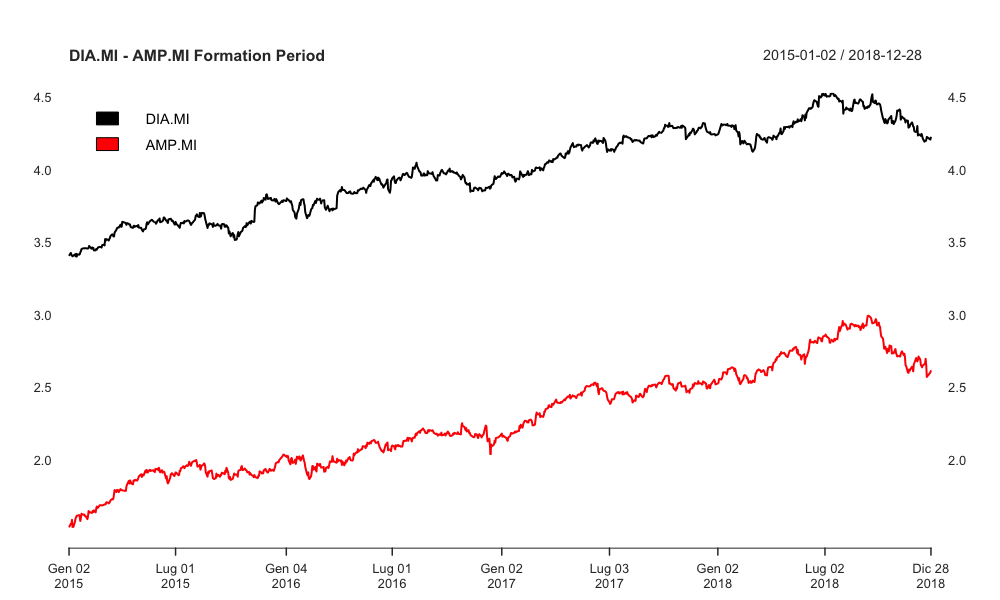
\includegraphics[width=0.7\textwidth]{dia_amp_logprezzi.png}%
		}
		
		\subfigure[$\Delta$ del logaritmo naturale dei prezzi ]{%
			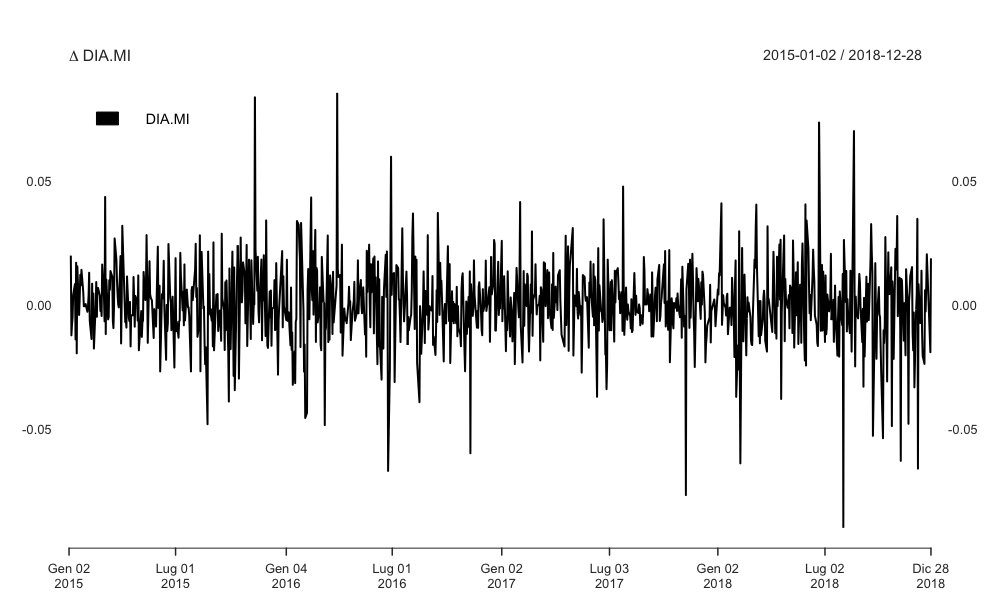
\includegraphics[width=0.7\textwidth]{dia_diff.png}%
		}
		\caption{\textbf{Formation Period}}
		\label{form_period}
\end{figure}
\
\begin{table}[H]

	\caption{Test di radice unitaria per i titoli nel \textit{formation period}}
	\begin{minipage}{.4\textwidth}
			\centering
		\caption{Prezzi}
		\begin{tabular}{@{}lll@{}}
			\toprule
			Tickers & ADF Statistic & p-value \\ \midrule
			DIA.MI  & -2.23         & 0.48    \\
			AMP.MI  & -1.89         & 0.62    \\
			UCG.MI  & -1.4          & 0.83    \\
			BPE.MI  & -2.45         & 0.39    \\
			BMED.MI & -1.19         & 0.90    \\
			BGN.MI  & -1.89         & 0.63    \\
			AZM.MI  & -2.35         & 0.43    \\ \bottomrule
		\end{tabular}
	\end{minipage}
    \begin{minipage}{.7\textwidth}
    	\centering
		\caption{logaritmo naturale dei prezzi}
		\begin{tabular}{@{}lll@{}}
			\toprule
			Tickers & ADF Statistic & p-value \\ \midrule
			DIA.MI  & -2.27         & 0.46    \\
			AMP.MI  & -2.06         & 0.55    \\
			UCG.MI  & -1.53         & 0.78    \\
			BPE.MI  & -2.47         & 0.38    \\
			BMED.MI & -2.44       & 0.39    \\
			BGN.MI  & -1.91         & 0.62    \\
			AZM.MI  & -2.04         & 0.56    \\ \bottomrule
		\end{tabular}
	\end{minipage}
	\label{tit_staz}
\end{table}
\
\\
\\
Il test ADF è stato effettuato  sui prezzi e sul logaritmo naturale dei prezzi delle serie storiche nel \textit{formation period}, nei livelli e nelle differenze. Come mostrato nelle tabelle \ref{tit_staz} e \ref{tit_diff_staz} l’ipotesi della presenza di radici unitarie trova ampia conferma negli esiti del test. I titoli scelti, mantengono la proprietà di integrazione, sono cioè non stazionari nei livelli ma stazionari nelle prime differenze.


\begin{table}[H]
	
	\caption{Test di radice unitaria per per le differenze dei titoli nel \textit{formation period}}
	\begin{minipage}{.4\textwidth}
		\centering
		\caption{Prezzi}
		\begin{tabular}{@{}lll@{}}
			\toprule
			Tickers & ADF Statistic & p-value \\ \midrule
			DIA.MI  & -9.75         & $\le$0.01    \\
			AMP.MI  & -10.16        &$\le$0.01    \\
			UCG.MI  & -9.96         &$\le$0.01    \\
			BPE.MI  & -10.59        & $\le$0.01    \\
			BMED.MI & -9.92         & $\le$0.01    \\
			BGN.MI  & -9.91         & $\le$0.01    \\
			AZM.MI  & -10.16        & $\le$0.01    \\ \bottomrule
		\end{tabular}
	\end{minipage}
	\begin{minipage}{.7\textwidth}
		\centering
		\caption{logaritmo naturale dei prezzi}
	\begin{tabular}{@{}lll@{}}
		\toprule
		Tickers & ADF Statistic & p-value \\ \midrule
		DIA.MI  & -10.19        & $\le$0.01    \\
		AMP.MI  & -10.68        & $\le$0.01    \\
		UCG.MI  & -9.84         & $\le$0.01    \\
		BPE.MI  & -10.68        & $\le$0.01    \\
		BMED.MI & -9.94         & $\le$0.01    \\
		BGN.MI  & -10.09        &$\le$0.01    \\
		AZM.MI  & -10.41        & $\le$0.01    \\ \bottomrule
	\end{tabular}
	\end{minipage}
\label{tit_diff_staz}
\end{table}
\
\\
La Tabella \ref{selezione} mostra i risultati della selezione ottenuta mediante i passaggi precedentemente discussi.
\\
I valori della statistica test ADF ci portano a rifiutare, per tutte le coppie considerate nel \textit{formation period}, l'ipotesi nulla di presenza di radice unitaria e quindi a considerare le combinazioni come processi stazionari.

\begin{center}
\captionof{table}{Risultati}\label{selezione}
\begin{tabular}{ p{4cm}p{1cm}p{2cm}p{1cm}p{3cm} }
	\hline
	Pair & $\rho$ & ADF Statistic & p-value & Settore\\
	\hline
	DIA.MI - AMP.MI  & 0.97  & -3.66 &  0.026 & Sanitario\\
	UCG.MI - BPE.MI & 0.94 & -3.73 & 0.022 & Bancario\\
	BMED.MI - BGN.MI & 0.80 & -4.43 & 0.01 & Servizi Finanziari \\
	BMED.MI - AZM.MI  & 0.61 & -3.98 & 0.01 & Servizi Finanziari\\
	\hline
\end{tabular}
\end{center}
%%%%%%%%%%
%%%%%%%%%%%
%%%%%%%%%%
%%%%%%%%%%%
%%%%%%%%%%
%%%%%%%%%%%


\subsection{Il modello operativo e la stazionarizzazione del \textit{trading period}}

Il modello operativo costruito per la strategia di Pair trading è formato da tre diverse metodologie, ciascuna di queste assume una diversa natura e un diverso processo di stazionarizzazione del \textit{trading period}.
Le tre metodologie sviluppate sono
\begin{itemize}
	\item \textbf{Approccio classico di cointegrazione}
	\item \textbf{Kalman Filter}
	\item \textbf{Rolling Regression}
\end{itemize}

\subsubsection*{Approccio classico di cointegrazione}

Il primo approccio, assume che una volta stimato il vettore di cointegrazione $\hat{\beta}$ nel \textit{formation period} questo possa rendere stazionaria la combinazione lineare dei due titoli nel \textit{trading period}. 
Come mostrato nella Eq. \ref{classic_co} il vettore di cointegrazione, per ogni nuova osservazione del periodo di trading, deve restituire una combinazione lineare il cui valore $z_t$, unito a quelli precedenti, costituisce una serie storica stazionaria.

\begin{equation}\label{classic_co}
	\begin{rcases}
		t=1 \qquad z_{1} = \ln(y_1) - \hat{\alpha} - \hat{\beta}\ln(x_1) \\
		t=2 \qquad z_{2} = \ln(y_2) - \hat{\alpha} - \hat{\beta}\ln(x_2) \\
		\cdots    \qquad \qquad \qquad \cdots  \qquad \qquad \qquad \cdots \\
	t=252 \qquad z_{252} = \ln(y_{252}) - \hat{\alpha} - \hat{\beta}\ln(x_{252}) \\
	\end{rcases}
\end{equation}
\\
I fattori che possono incidere sull’efficacia della stazionarizzazione del trading period ottenuta mediante l’Eq. \ref{classic_co}, hanno una duplice natura. Da un lato è necessaria l’individuazione del vero vettore di cointegrazione, infatti una stima distorta conduce ad uno scarso risultato in termini di stazionarietà. Dall’altro la condizione necessaria è legata alla persistenza della relazione di cointegrazione. Sebbene la persistenza della relazione di cointegrazione tra due serie storiche sia possibile, nella pratica e quindi nel mercato azionario tale proprietà è raramente presente, come dimostrato dagli studi condotti da Clegg(2014).

\subsubsection*{Kalman Filter}
L'utilizzo di modelli nello spazio degli stati e del filtro ricorsivo di Kalman, ha trovato negli anni numerosi campi di applicazione. Dai sistemi di tracciamento balistico all'utilizzo nella decomposizione e analisi delle serie storiche, il Kalman Filter fornisce un efficiente valutazione di un sistema dinamico soggetto a rumori.
Modelli tipici di Linear State Space Models, ampiamente utilizzati nell'analisi econometrica delle serie storiche sono : \textbf{Local Level Model, Time series decomposition, Time series seasonality.}
L'assunzione alla base del Kalman Filter è che il vettore di cointegrazione $\hat{\beta}$ si aggiorni nel tempo con l'introduzione di nuove informazioni, nella pratica l'utilizzo del Kalman Filter in questo lavoro è stato quello di tracciare l'evoluzione di $\alpha$ e $\beta$,come mostrato nell'Eq. \ref{kalman_eq},allo scopo di verificare la stazionarietà della serie storica.


\begin{equation}\label{kalman_eq}
	\begin{rcases}
		t=1 \qquad z_{1} = \ln(y_1) - \hat{\alpha_0} - \hat{\beta_0}\ln(x_1) \\
		t=2 \qquad z_{2} = \ln(y_2) - \hat{\alpha_1} - \hat{\beta_1}\ln(x_2) \\
		\cdots    \qquad \qquad \qquad \cdots  \qquad \qquad \qquad \cdots \\
		t=252 \qquad z_{252} = \ln(y_{252}) - \hat{\alpha_{251}} - \hat{\beta_{251}}\ln(x_{252}) \\
	\end{rcases}
\end{equation}
\\

\subsubsection*{Rolling Regression}
Il terzo approccio segue fedelmente l'idea alla base dell'utilizzo di un \textbf{Linear State Space Model}, ossia che l'assunzione dell'approccio classico di cointegrazione sia quantomeno poco ragionevole nell'ottica dei mercati finanziari.
A tale scopo è stato scelto di utilizzare una regressione lineare con finestra mobile o \textit{Rolling Regression}. Ciò vuol dire che nel \textit{trading period} a intervalli di 2 mesi (40 giorni di quotazioni), i parametri $\alpha$ e $\beta$ sono stati ristimati e utilizzati per generare il processo nei 2 mesi successivi. 


\subsection{Definizione della strategia di trading}
Una volta identificata la relazione di cointegrazione che lega l’andamento dei prezzi
di due titoli e specificata la struttura del modello operativo per le diverse metodologie utilizzate procediamo alla definizione della strategia di investimento. 
\\
Una volta identificato il vettore cointegrante, la combinazione lineare

\begin{equation} 
	z_t= \ln(stock_{1,t}) - \hat{\beta}\ln(stock_{2,t}) - \hat{\alpha} \label{spread}
\end{equation}
\
\\
è un processo stazionario che tenderà ad oscillare attorno al suo valore medio.
\\
Questa caratteristica, definita come \textit{mean reversion} di un processo stazionario, ci permette di definire la strategia operativa che utilizzeremo.
Ipotizziamo di fissare due bande che rappresentino un limite inferiore e un limite superiore per le fluttuazioni della combinazione linare $z_t$,la rottura di una delle due bande costituisce un segnale di entrata (\textit{long o short}) per il modello(quindi un oscillazione del processo lontana dal suo valore medio), mentre la chiusura delle posizioni aperte avviene in corrispondenza del ritorno al valore medio del processo. 


\subsubsection{Costruzione della threshold}
La letteratura relativa alla scelta delle thresholds in una strategia di \textit{pair trading} è ampia e diversificata.
Gatev et al.(2006) nel loro lavoro, adottano come threshold (valore soglia) per una strategia di pair trading un valore pari a 2 volte la deviazione standard dello spread calcolato nel \textit{formation period}.
Tuttavia un problema dell'adottare una threshold con l'approccio di \textit{Gatev et al.} risiede nel considerare una soglia eccessivamente alta per le oscillazioni nel \textit{trading period}, portandoci nella maggior parte dei casi a non avere segnali di entrata o uscita.
Lavori più recenti adottano come thresholds per i segnali di entrata e uscita, stime rolling della volatilità del processo di spread, ad esempio attraverso modelli per la volatilità condizionata (GARCH).
Questo approccio risulta piuttosto valido in quanto tiene conto dell'evoluzione della variabilità del processo nel \textit{trading period},adattandosi a possibili shock nella quotazione dei titoli.
Altri lavori adottano metodi più "classici",utilizzando il 5° e il 95° percentile (rispettivamente la soglia inferiore e la soglia superiore) del processo stimato nel \textit{formation period}.
Nella nostra casistica è stato scelto di adottare un valore soglia prefissato e costante per tutte le metodologie sviluppate.
Tale scelta ha due motivazioni:
\begin{enumerate}
	\item Riuscire ad equiparare le performance di tutti i modelli
	\item Generari segnali aggressivi di entrata per tutti i modelli
\end{enumerate}

Come visto la scelta della \textit{threshold} di operatività è fondamentale in una strategia di questo genere. Sebbene il nostro intento prescinda dal valutare quale metodologia sia più profittevole (anzi valutiamo il rischio connesso a questa strategia) la scelta di un valore soglia che produca segnali aggressivi è motivata da ottenere maggiori informazioni da valutare dal punto di vista statistico.

\subsubsection{Generazione dei segnali operativi}
Dopo aver individuato la soglia superiore e la soglia inferiore illustriamo la dinamica che a seguito della rottura di uno questi due limiti genera un segnale operativo.
\\
Definiamo con il termine \textit{threshold} il valore soglia scelto, per cui avremo che 
\\
\begin{itemize}
	\item Se : \textbf{$z_t > threshold$} . significa che $stock_{1,t}$ è sopravvalutato rispetto a $stock_{2,t}$, per cui vendiamo 1 unità di $stock_{1,t}$ e compriamo $\hat{\beta}$ unità di $stock_{2,t}$
	Chiudiamo la posizione quando $z_t\leq 0$
	\item Se: \textbf{$z_t < - threshold$} . significa che $stock_{1,t}$ è sottovalutato rispetto a $stock_{2,t}$, per cui compriamo 1 unità di $stock_{2,t}$ e vendiamo $\hat{\beta}$ unità di $stock_{1,t}$
	Chiudiamo la posizione quando $z_t\geq 0$
\end{itemize}
\
\\
La rottura della soglia superiore, che definiamo come \textit{threshold long} nella strategia, genera un segnale operativo uguale a \textbf{-1}. Specularmente la rottura della \textit{threshold short} genera un segnale operativo uguale a \textbf{+1}.
Questa logica per la generazione dei segnali risulta più chiara alla luce della prossima sezione.

\subsubsection{Costruzione del portafoglio}
\
L'intera strategia di trading è equivalente ad avere un portafoglio con pesi\footnote{Yiyong Feng and Daniel P. Palomar (2016), "A Signal Processing Perspective on Financial Engineering"}
\begin{equation} 
w\triangleq 
\begin{bmatrix}
	1 \\
	-\hat{\beta}
\end{bmatrix}
\end{equation}
\
\\
Ciò vuol dire che nel momento in cui il processo oltrepassa la \textit{threshold long}, il segnale generato, corrispondente a \textbf{-1} calibrerà il portafoglio in modo da acquistare, per il giorno successivo alla generazione del segnale, $\hat{\beta}$ unità dello stock 2, (avremo $ + \hat{\beta}$ unità) e vendere 1 unità dello stock 1, (avremo -1 unità) .
I pesi del portafoglio risulteranno speculari nel caso in cui il processo oltrepassa la soglia definita come \textit{threshold short}.
Avremo che il giorno successivo alla generazione del segnale, il portafoglio sarà costituito da $- \hat{\beta}$ unità dello stock 2, unità) e +1 unità dello stock 1.
\\
Sotto il vincolo che $ \mathbf{\lVert w \rVert =1}  $ il portafoglio costruito per la strategia è :

\begin{equation} 
w\triangleq \begin{bmatrix}
	1/(1 + \hat{\beta}) \\
	-\hat{\beta}/(1 + \hat{\beta})
\end{bmatrix}
\end{equation}
\
mentre i rendimenti delle due posizioni sono stati poi calcolati come
\begin{equation}
	w^T\Delta \ln(stocks)
\end{equation}

mentre il rendimento totale del portafoglio è il differenziale del rendimento tra le due posizioni.

\subsubsection*{Una strategia long-short}

Il portafoglio costruito mediante questo modello operativo rientra nella categoria delle strategie definite \textit{long-short}.
Le motivazioni che spingono la scelta di andare lunghi su un asset e contestualmente corti su un altro asset possono essere diverse.
In generale un portafoglio costruito nell'ambito di una strategia \textit{long-short}, presenta una esposizione minima nei confronti del mercato e rendimenti incorrelati rispetto allo stesso, ciò perchè il controvalore della posizione corta su uno dei due titoli, fornisce un ammontare utile a coprire, in modo totale o parziale, l'utile generato dalla posizione lunga sull'altro asset.
La peculiarità di assumere posizioni di segno opposto su diversi strumenti finanziari permette che il portafoglio abbia una esposizione pressochè nulla rispetto ad ampi movimenti del mercato.
Strategie di questo tipo si collocano tra le cosiddente \textit{market neutral strategies}.


\subsection{\textit{Trading} Performance}

\subsubsection{Premesse al modello}
Il modello operativo che è stato costruito durante questo lavoro è stato poi testato nel \textit{trading period}, ossia il periodo successivo al \textit{formation period}.
Nel nostro lavoro di \textit{Back Testing} della strategia è necessario però fare delle premesse, assumiamo cioè che valgano le
seguenti condizioni

\begin{enumerate}
	\item Nell'analisi della \textit{trading performance} non esistono costi di transazioni, questo elimina l'onere di considerare fattori come il \textit{bid-ask spread} , commissioni applicate dai broker e lotti minimi di negoziazione.
	\item Nell'ipotesi di rottura del legame di cointegrazione non vi è un intervento nella strategia.
\end{enumerate}

L'assunzione di queste condizioni agevola lo svolgimento del lavoro di analisi del modello operativo. Come evidenziato precedentemente, la scelta di determinati assets è legata alle dinamiche seguite dall'evoluzione temporale delle loro serie storiche, e non alla particolarità degli aspetti tecnici che caratterizzano,ad esempio, la loro negoziazioni. Di fatto l'implementazione della strategia per i diversi assets considerati avverrà assumendo un \textit{environment} semplificato, che non considera molti aspetti del mercato borsistico.
La scelta di non intervenire nel caso di rottura del legame di cointegrazione appare ragionevole alla luce della "non conoscenza" del trader dell'effettiva rottura del legame. 
\subsubsection{Analisi della performance}

La misurazione delle prestazioni è una componente cruciale del trading algoritmico. Senza una valutazione delle prestazioni, insieme a una solida tenuta dei registri, è difficile, se non impossibile, determinare se i profitti di una strategia sono dovuti alla fortuna o a causa di un certo margine sul mercato.
In un sistema automatico di trading sono diversi gli aspetti da valutare a diversi livelli di granularità. Ciò è quantomeno importante per individuare i punti di forza e debolezza nella strategia costruita.
Quando valutiamo quindi la performance di una strategia relativa ad un portafoglio in un periodo nel passato ( metodi sistematici di valutazione di una strategia nel passato prendono il nome di \textit{Back Testing}, ciò che vogliamo verificare è

\begin{enumerate}
	\item Se le regole sistematiche codificate dalla strategia producono effettivamente un rendimento e se la strategia possiede prestazioni positive nel backtesting.
	\item Le prestazioni di differenti strategie / portafogli, al fine di valutare quale strategia possa essere più efficace.
\end{enumerate}

A tal fine possiamo distinguere due principali aspetti nella valutazione di performance:

\begin{itemize}
	\item Analisi dei rendimenti della strategia
	\item Analisi Rischio/Rendimento
\end{itemize}
\
\\
L’aspetto più visibile di una strategia di trading  è la percentuale di profitto rispetto al capitale iniziale, in un ambiente di backtesting o di live trading. Diverse sono gli strumenti utilizzati nell'analisi dei profitti, da strumenti grafici come la cosiddetta \textit{Equity Line}, che fornisce una stima del comportamento del sistema nel tempo a misure di rendimenti come il \textit{Total Return}(Rendimento totale) o misure di rendimento composto quali il \textit{Compound Annual Growth Rate (CAGR)}.
L'analisi del grafico di una performance è però non da considerare in maniera assoluta,  guardando rapidamente dove si conclude
nel tempo, bensì  bisogna valutarne la variabilità cosiderando che il sistema
ideale produrrà un equity line a 45 gradi il meno variabile possibile.
L’equity line rappresenta quindi il primo step che un sistema deve superare,
la sua analisi è veloce e grafica ma deve comunque essere effettuata con
attenzione.
\\
La misurazione del rischio, che è quasi inseparabile dalla
valutazione delle prestazioni, è diventata ormai multidimensionale nel tentativo di rispondere a  una semplice domanda: "Quanto potrei perdere?".
La costruzione del portafoglio e la gestione del rischio connesso ad un portafoglio sono di fatto due lati della stessa medaglia, per cui la domanda più appropriata sembrerebbe essere
"Come posso massimizzare il mio profitto ed evitare di andare in rovina?".
\\
Sebbene il concetto di "rischio" possa avere degli aspetti soggettivi (basti pensare che i fondi di investimento spesso misurano l'investimento rispetto al profilo di rischio del titolare del portafoglio), nel mondo della finanza è lecito considerare che ogni investitore sia sostanzialmente \textit{avverso al rischio} in quanto,questo,a parità di rendimento  sceglierà sempre il portafoglio meno rischioso o che in un ottica di guadagno sicuro preferisce avere meno rischi.
Parlare del rischio in modo puramente descrittivo è utile ed istruttivo ma non è sufficiente. Il rischio deve essere quantificato. Più precisamente, il rischio del portafoglio di un investitore deve essere misurato.
In questo lavoro ci concentreremo prevalentemente sull'analisi dei rischi di un portafoglio finanziario, per farlo ci avvarremo di strumenti statistico-finanziari di valutazione del rischio.
\\
Nei prossimi paragrafi saranno trattati nel dettaglio le misure utilizzate.

\subsubsection*{Sharpe Ratio}
Lo Sharpe Ratio (SR) o Indice di Sharpe,così chiamato in onore del premio Nobel per l'economia 1990 William Sharpe,
viene definito come il rapporto tra la media dei rendimenti in eccesso rispetto alla media dei rendimenti di un titolo privo di rischio e la deviazione standard dei rendimenti stessi. Rappresenta perciò una misura del \textit{trade-off} tra rendimento e rischio di un portafoglio o meglio misura il rendimento per unità di rischio. Maggiore è l'indice di Sharpe, migliore è la performance combinata di "rischio" e rendimento.

\begin{equation}
	SR = 
	\frac{\E{[r_t]}-\E{[r_{ft}]}}{\sigma}
\end{equation}

Sebbene sia largamente impiegato nella prassi, e fornisca una giustificazione immediata al modello di equilibrio di riferimento per i mercati finanziari, il Capital Asset Pricing Model, l'indice di Sharpe non è immune da critiche.
Niente infatti implica che il rischio, un concetto per sua natura soggettivo, debba coincidere con la varianza (o, in maniera equivalente, con la deviazione standard) del rendimento; questo tipo di obiezione è analogo a quelle mosse alla teoria della frontiera dei portafogli con preferenze di tipo media-varianza. La riflessione sull'idoneità dell'indice di Sharpe a rappresentare le preferenze degli operatori finanziari ha portato allo sviluppo di misure di performance alternative che piuttosto che utilizzare come misura per il rischio la deviazione standard, utilizzano misure come il VaR o l'ES.
In questo lavoro utilizzeremo misure di rischio annualizzate, nello specifico lo Sharpe Ratio che andremo a considerare sarà uno Sharpe Ratio annualizzato(ASR)

\begin{equation}
	ASR = 
	\frac{\E{[r_t]}-\E{[r_{ft}]}}{\sigma}\sqrt{252}
\end{equation}

\subsubsection*{Max Drawdown}

Il drawdown di un portafoglio finanziario è la perdita generata in un dato orizzonte temporale di investimento. È una misura del declino da un massimo relativo storico ad un minimo relativo seguente,  e la più grande escursione di questo tipo, nel periodo considerato, prende il nome di massimo drawdown.
La soglia di "sopportazione" o per meglio dire la gestione dei periodi di drawdown di un portafoglio finanziario è una scelta che attiene al profilo di rischio personale dell'investitore.
L'esposizione alle perdite è quindi un fattore che potremmo classificare come "soggettivo" in una strategia di trading.
Un esposizione prolungata, sebbene con drawdowns minori può essere nell'ottica dell'investitore una sofferenza eccessiva a fronte del profitto atteso.
In questo lavoro oltre a riportare il massimo drawdown ottenuto dai portafogli, analizzeremo lunghezza (in termini giornalieri) e profondità delle perdite registrate.


\subsubsection*{Compounded Returns}
Il P\&L complessivo è stato calcolato come rendimento composto, ciò vuol dire che tutta la ricchezza esistente al momento t è reinvestita.
\
\\
In termini più formali 
\begin{equation}
	prod(1 + R) - 1
\end{equation}

\subsubsection*{Root Mean Squared Error}
Al fine di poter valutare la qualità della stima , da un punto di vista statistico,dei diversi metodi utilizzati è stato scelto di calcolare una misura di perdita quadratica. Nello specifico è stata considerata la radice quadrata dell'errore quadratico medio( RMSE ) ed è stato calcolato come segue:

\begin{equation}
	RMSE = \sqrt{\frac{\sum_{i=1}^{n}(y_i - \hat{y_i})^2}{n}}
\end{equation}
\\
dove $i=1....n$ è riferito al \textit{periodo di trading} e $\hat{y_i}$ è la stima dello $stock_{1,i}$ ottenuta come:
\begin{equation}
	stock_{1,i} = \hat{\alpha} + \hat{\beta} stock_{2,i}\footnote{il RMSE è stato calcolato sui logaritmi dei prezzi degli assets.}
\end{equation}
\\
considerando $\alpha$ e  $\beta$ ottenuti con i diversi metodi.
Un analisi di questo tipo di misura ci permette di quantificare da un punto di vista statistico l'efficacia dei modelli nel \textit{trading period}.


\subsubsection*{Value-at-Risk}

Il value at risk (VaR) è un indicatore di rischio utilizzabile nelle decisioni finanziarie. Esso esprime la perdita massima probabile (a un certo livello di confidenza statistica) in un determinato orizzonte temporale.
La definizione di VaR giornaliero, espresso in termini di rendimento, ad un livello $\alpha$ di probabilità è
\begin{equation}
	Pr[X_{t+1} \le - VaR_{t+1}^{\alpha}] = \alpha
\end{equation}
In termini più formali il VaR a livello di probabilità $\alpha$ (es. 95\%) è il quantile di livello $\alpha$ dei rendimenti negativi, o equivalentemente,
è il valore negativo del quantile $1- \alpha$ dei rendimenti.
\begin{equation}
	VaR_{\alpha}(X) = - q_{\alpha}(X)
\end{equation}
\
\\
Il VaR che andremo a considerare sarà un VaR annualizzato, ossia moltiplicato per la radice dell'orizzonte temporale utilizzato nel \textit{trading period}, cioè 252 giorni di mercato.
Sotto l'ipotesi che i rendimenti delle performance seguano una distribuzione normale, quindi $R \sim \mathcal{X}(\mu,\sigma)$ la definizione del VaR è la seguente

\begin{equation}
	VaR_{\alpha}(X)=  - \mu \cdot \Phi^{-1} \cdot \sigma
\end{equation}
\
dove $\Phi^{-1}$ è il quantile di livello $\alpha$ di una normale standardizzata.


\subsubsection*{Expected Shortfall}

L'Expected Shortfall (ES) è una misura di rischio che prende in considerazione sia la probabilità di subire perdite superiori al VaR sia la loro dimensione.
\\
Viene definito come il valore atteso della perdita dato che questa è superiore al VaR.
L'ES giornaliero di un portafoglio finanziario, in termini di rendimento è definito come

\begin{equation}
	ES_{\alpha}(X)= \frac{1}{\alpha} \int_{0}^{\alpha} VaR_u(X)du
\end{equation}
\
Se assumiamo che i rendimenti del portafoglio seguano una distribuzione normale la definizione di Expected Shortfall sotto condizione di normalità è la seguente

\begin{equation}
	ES_{\alpha}(X) = \frac{\phi(\Phi^{-1})}{\alpha} \cdot \sigma
\end{equation}
\
dove $\phi(x)$ è la funzione di densità di una distribuzione normale standard.
%%%%%%%%%%
%% RISULTATI EMPIRICI
%%%%%%%%%%
\subsection{Risultati Empirici}

Il paragrafo che segue sintetizza i risultati ottenuti applicando il modello operativo.
A tale scopo è stata sviluppata una duplice analisi

\begin{itemize}
	\item \textbf{Analisi dei processi}
	\item \textbf{Analisi Trading Performance}
\end{itemize}
\
\\
La prima tipologia di analisi è stata effettuata allo scopo di individuare le criticità ,delle tre metodologie sviluppate, nella costruzione di un processo stazionario per il \textit{trading period}. La stazionarietà del processo, garantisce che il fenomeno sia \textit{mean reverting}, condizione che a sua volta costituisce l'elemento ideale per l'implementazione di una strategia di Pair Trading.
A tal fine abbiamo abbiamo effettuato un'analisi sulla stazionarietà dei processi generati $S_{1,T},S_{2,T},S_{3,T}$.
In altre parole abbiamo testato la capacità del vettore di cointegrazione di rendere stazionaria la combinazione lineare ottenuta mediante i valori del trading period. Anche in questo caso siamo ricorsi al test ADF.
\\
La seconda tipologia di analisi tenta di individuare, da un punto di vista finanziario, criticità e punti di forza di una strategia di Pair trading basata su tre differenti approcci.
A tale scopo è stato effettuata un analisi di Back Testing.
Per fare questo si è collocato il punto di osservazione alla fine del \textit{trading period}, guardando indietro sono state rilevate le operazioni eseguite dal nostro modello fino a quel momento, valutandone i risultati in termini di rischio e rendimento.

\break
\subsection*{Diasorin S.p.A. - Amplifon S.p.A.}

La prima coppia considerata (in ordine di correlazione) è formata dalle multinazionali \textbf{DiaSorin S.p.A.} e  \textbf{Amplifon S.p.A.}, entrambe operanti nel settore medico-sanitario.

\begin{center}
	\captionof{table}{Analisi dei processi, DIA.MI- AMP.MI}\label{stazionarietà_dia_amp}
	\begin{tabular}{ p{2cm}p{3cm}p{1cm}p{2cm}p{1cm}}
		\hline
		Processo & Metodologia & ADF Statistic & p-value & RMSE \\
		\hline
		$S_1$ & Cointegrazione & -3.55 & 0.041 & 0.037 \\
		$S_2$ & Kalman Filter & -5.01 & 0.01  & 0.013\\
		$S_3$ & Rolling Regression & -3.70 & 0.020 & 0.032  \\
		\hline
	\end{tabular}
\end{center}
\
\\
I risultati delle statistiche test  in tabella \ref{stazionarietà_dia_amp} ci mostrano come per tutti i metodi considerati i valori assunti dal vettore di cointegrazione $\beta^*$ riescano a rendere stazionarie le serie nel \textit{trading period}.
\\
La Tabella \ref{performance_dia_amp} mostra come il metodo vincente in un ottica di solo profitto risulti essere il metodo di \textbf{Rolling Regression} sebbene in questo caso, come anche nel caso del metodo di \textbf{Cointegrazione} l'implementazione della strategia potrebbe diventare rischiosa. Soprattutto nel caso in cui il processo si trovi oltre una certa soglia, verrebbe meno il vantaggio derivante dal prevedibile ritorno verso la media.
Osserviamo che  i risultati del \textit{VaR} e dell'\textit{ES} ci suggeriscono che  ad un livello di confidenza del 95\% la metodologia che subisce minori perdite è il \textit{Kalman Filter}.
Ciò potrebbe essere esteso alla natura dello spread calcolato attraverso l'utilizzo di vettori di cointegrazione stimati dinamicamente.
La natura meno \textit{"random walk"} della combinazione lineare ottenuta nel \textit{trading period} e la componente fortemente stazionaria, come evidenziato dall'analisi dei processi in tabella \ref{stazionarietà_dia_amp}, suggerisce che un portafoglio così costruito sia meno soggetto a variazioni estreme nella coda sinistra della distribuzione.

% PERFORMANCE
\begin{center}
	\captionof{table}{Analisi trading performance, DIA.MI-AMP.MI}\label{performance_dia_amp}
	\begin{tabular}{ p{3cm}p{2cm}p{2cm}p{2cm}p{1cm}p{1cm}}
		\hline
		Metodologia  & Sharpe Ratio & Max Drawdown & Returns & VaR & ES\\
		\hline
		Cointegrazione & 2.61 & 0.051 & 0.39 & 0.28 & 0.32\\
		Kalman Filter & 2.01 & 0.025 & 0.24 & 0.24 & 0.28   \\
		Rolling Regression & 3.16 & 0.051 & 0.47 & 0.26 & 0.30 \\
		\hline
	\end{tabular}
\end{center}
\
\\
\begin{center}
\begin{tabular}{@{}llll@{}}
	\toprule
	From       & To         & Drawdown   & Lunghezza \\ \midrule
	2019-01-03 & 2019-01-04 & -0.0218 & 2      \\
	\rowcolor[HTML]{FFCCC9} 
	2019-01-07 & 2019-01-29 & -0.0519 & 17     \\
	2019-05-27 & 2019-06-06 & -0.0275 & 9      \\
	2019-08-13 & 2019-10-03 & -0.0227 & 37     \\
	2019-10-08 & 2019-11-22 & -0.048  & 34     \\ \bottomrule
\end{tabular}
	\captionof{table}{Analisi Drawdowns,Cointegrazione}\label{drawdowns_dia_amp_coint}
\end{center}
\
\\
\begin{center}
	\begin{tabular}{@{}llll@{}}
		\toprule
		From       & To         & Drawdown  & Lunghezza \\ \midrule
		2019-01-18 & 2019-03-06 & -0.0366 & 34     \\
		2019-03-27 & 2019-04-23 & -0.0189 & 18     \\
		2019-05-27 & 2019-06-19 & -0.0277 & 18     \\
		2019-07-01 & 2019-09-19 & -0.0239 & 58     \\
		\rowcolor[HTML]{FFCCC9} 
		2019-11-15 & NA         & -0.0456 & 30     \\ \bottomrule
	\end{tabular}
	\captionof{table}{Analisi Drawdowns,Kalman Filter}\label{drawdowns_dia_amp_kf}
\end{center}

\
\\
\begin{center}
	\begin{tabular}{@{}llll@{}}
		\toprule
		From       & To         & Drawdown   & Lunghezza \\ \midrule
		2019-01-03 & 2019-01-04 & -0.0218 & 2      \\
		\rowcolor[HTML]{FFCCC9} 
		2019-01-07 & 2019-01-29 & -0.0519 & 17     \\
		2019-06-05 & 2019-08-01 & -0.0459 & 42     \\
		2019-10-24 & 2019-11-18 & -0.0262 & 18     \\
		2019-11-22 & 2019-12-17 & -0.0213 & 18     \\ \bottomrule
	\end{tabular}
	\captionof{table}{Analisi Drawdowns,Rolling Regression}\label{drawdowns_dia_amp_rl}
\end{center}
\
Nelle tabelle \ref{drawdowns_dia_amp_coint},\ref{drawdowns_dia_amp_kf},\ref{drawdowns_dia_amp_rl} vengono mostrati i drawdown delle performance per i tre modelli.
Il modello di approccio classico di cointegrazione registra un esposizione maggiore alle perdite in periodi brevi, ciò significa che in un lasso di tempo breve il portafoglio costruito con questo metodo registra uno stress maggiore al ribasso.
Il modello Kalman Filter sebbene registri periodi prolungati di drawdown, subisce anche minori perdite, con un max drawdown di circa  il \textbf{4\%} del valore del portafoglio
Le perfomance del modello di Rolling Regression,registrano invece un primo periodo di profondi drawdown, per poi stabilizzare l'esposizione alle perdite nel l'ultimo trimestre di \textit{trading period}.




\begin{figure}[htp]
	\begin{center}
	
	\subfigure[Kalman Filter spread]{%
		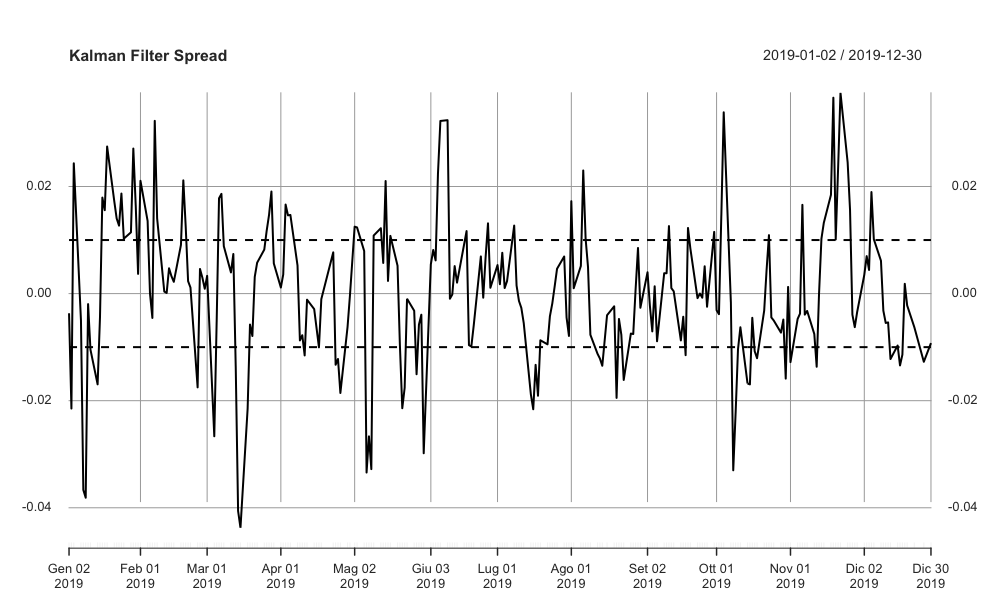
\includegraphics[width=.8\textwidth]{dia_amp_kfspread.png}%
	}
	
	\subfigure[Cointegration Spread]{%
		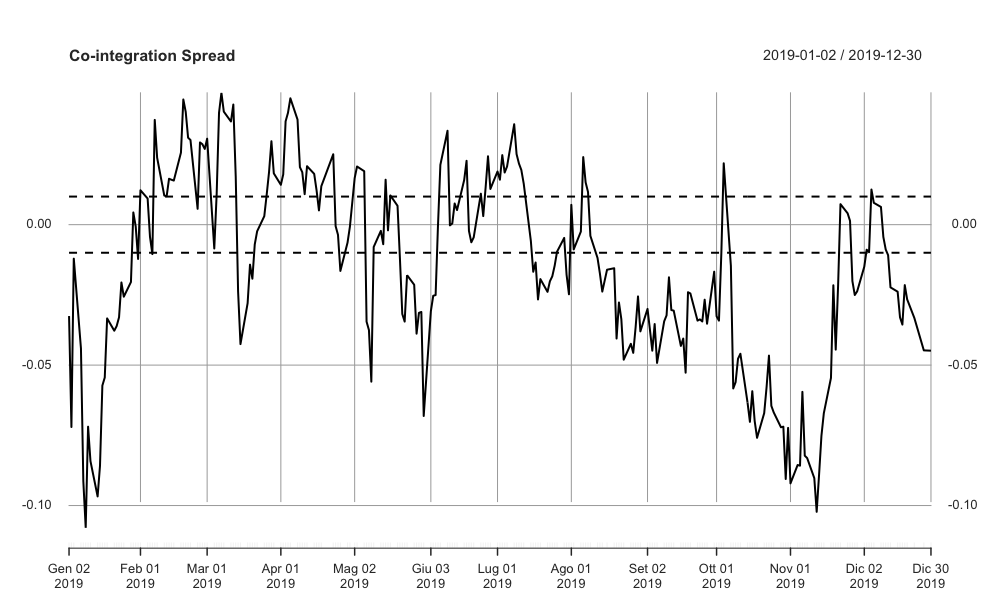
\includegraphics[width=.8\textwidth]{dia_amp_lsspread.png}%
	}
	\subfigure[Rolling Regression Spread]{%
		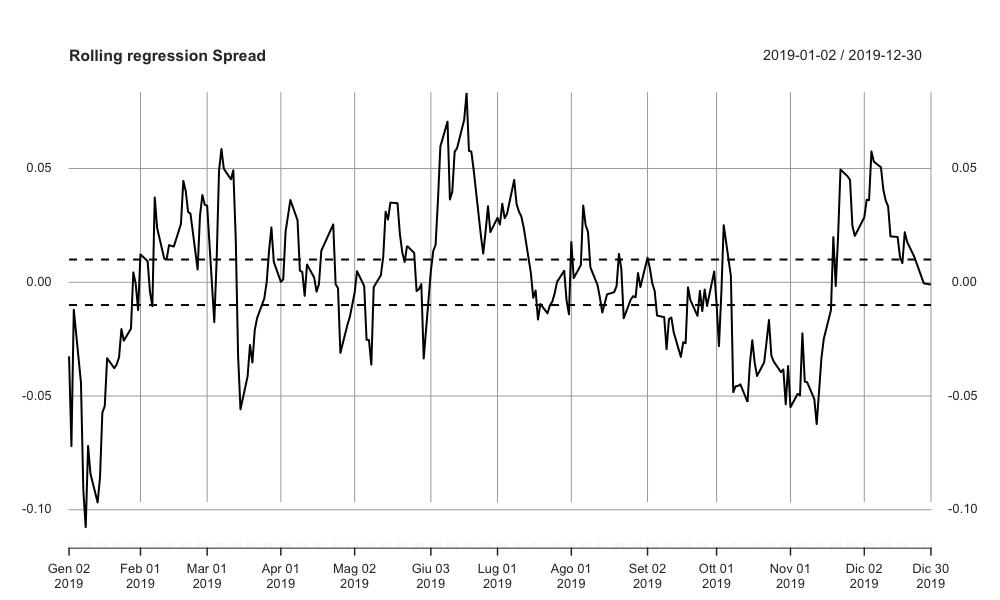
\includegraphics[width=.8\textwidth]{dia_amp_rlspread.png}%
	}
	\caption{\textbf{Spread per le tre metodologie,DIA.MI-AMP.MI}}
	
	\end{center}
\end{figure}


\
\begin{figure}[htp]
	\begin{center}
		
		\subfigure[\textbf{$\alpha$}]{%
			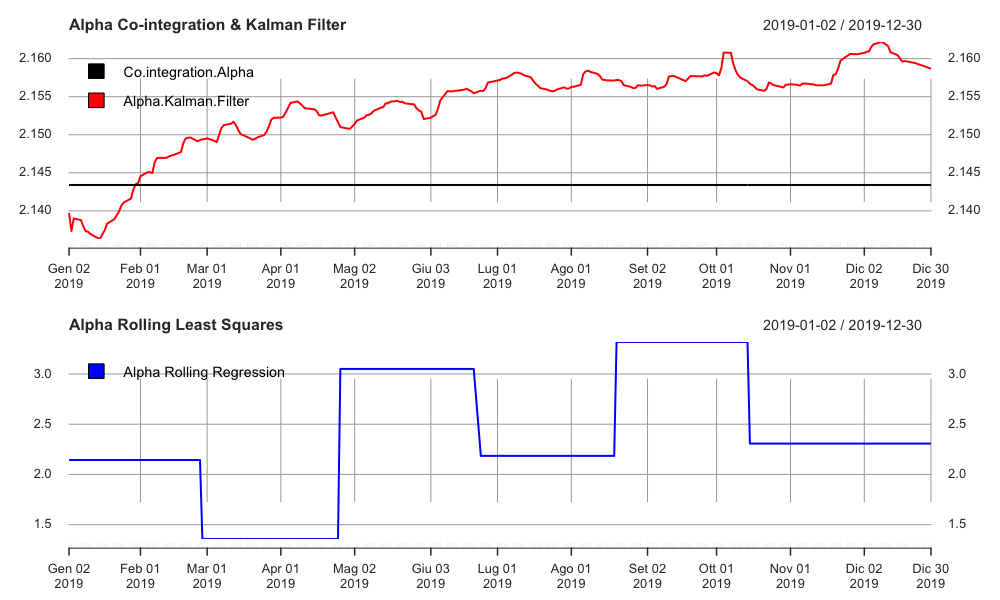
\includegraphics[width=.8\textwidth]{dia_amp_alpha.png}%
		}
		
		\subfigure[\textbf{$\beta$}]{%
			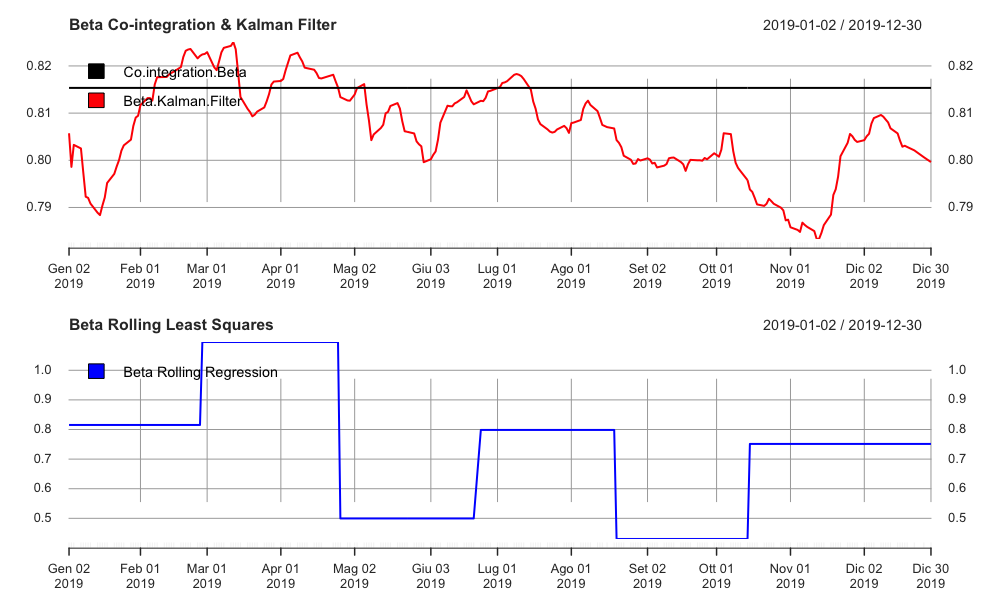
\includegraphics[width=.8\textwidth]{dia_amp_beta.png}%
		}

		\caption{\textbf{Alpha e Beta, DIA.MI - AMP.MI}}
		
	\end{center}
\end{figure}


\begin{figure}
	\centering
	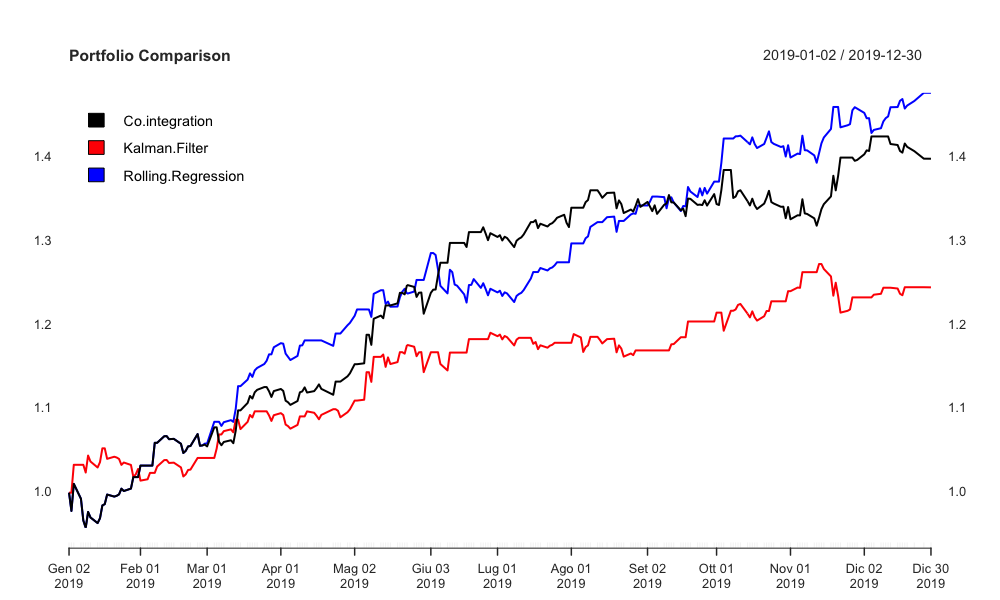
\includegraphics[scale=0.3]{dia_amp_portfolio.png}
	\caption{\textbf{P\&L, DIA.MI-AMP.MI}}
\end{figure}

\break
\break
\subsection*{Unicredit S.p.A. - Bper Banca S.p.A.}
La seconda coppia che è stata presa in considerazione è la coppia \textbf{Unicredit S.p.A. - Bper Banca S.p.A.} entrambi titoli appartenenti al settore Bancario.
I risultati presenti in tabella \ref{stazionarietà_ucg_bpe} mostrano uno scenario differente rispetto al caso di \textbf{Diasorin S.p.A. - Amplifon S.p.A}.
\\
I valori dell'ADF test ci mostrano come  i valori assunti dal vettore di cointegrazione $\hat{\beta}$ con il Linear State Space Model riescano a rendere stazionaria la serie $S_2$ nel \textit{trading period} ad un livello di significatività di $\alpha$ del 5\%. 
Il modello di Cointegrazione e il metodo della Rolling Regression risultano poco efficaci nel stazionarizzare il periodo di operatività. Ciò risulta ancora più visibile dall'analisi grafica dei processi ottenuti in figura \ref{spread_ucg_bpe}.
Osserviamo che per quanto riguarda l'efficacia dei modelli considerati, il Kalman Filter risulti essere quello che presenta un errore quadratico medio minore rispetto agli altri metodi considerati.

\begin{center}
	\captionof{table}{Analisi dei processi,UCG.MI-BPE.MI}\label{stazionarietà_ucg_bpe}
	\begin{tabular}{ p{2cm}p{3cm}p{1cm}p{2cm}p{1cm}}
	\hline
	Processo & Metodologia & ADF Statistic & p-value & RMSE \\
	\hline
	$S_1$ & Cointegrazione & -2.83 & 0.22 & 0.099 \\
	$S_2$ & Kalman Filter & -4.46 & 0.01  & 0.026 \\
	$S_3$ & Rolling Regression & -2.81 & 0.23 & 0.053 \\
	\hline
	\end{tabular}
\end{center}
\
\\
La Tabella \ref{performance_ucg_bpe} riassume la \textit{trading performance} ottenuta per la coppia Unicredit S.p.A- Bper Banca S.p.A.
Rilevante risulta essere che nell \textit{trading period} il modello Kalman Filter produce performance, in termini di rendimento del portafoglio, più basse rispetto ai modelli di Cointegrazione e Rolling Regression.
I risultati del VaR e dell'ES a un livello di confidenza del 95\% ci restituiscono uno scenario in cui ci aspettiamo che il Kalman Filter subisca minori perdite.

% PERFORMANCE
\begin{center}
	\captionof{table}{Analisi Performance Trading}\label{performance_ucg_bpe}
	\begin{tabular}{ p{3cm}p{2cm}p{1cm}p{1cm}p{1cm}p{1cm}}
	\hline
	Metodologia  & Sharpe Ratio & MDD & Returns & VaR & ES\\
	\hline
	Cointegrazione & 1.12 &  0.10 & 0.13  & 0.18 & 0.24  \\
	Kalman Filter & 1.01 & 0.074 & 0.02 & 0.16 &  0.21  \\
	Rolling Regression & 1.92 & 0.076 & 0.28  & 0.20 & 0.26  \\
	\hline
	\end{tabular}
\end{center}
\
\\\\\\\\
\begin{center}
\begin{tabular}{@{}llll@{}}
	\toprule
	From       & To         & Depth   & Length \\ \midrule
	2019-01-15 & 2019-02-08 & -0.0339 & 19     \\
	2019-04-10 & 2019-07-31 & -0.0738 & 78     \\
	2019-08-01 & 2019-08-19 & -0.0552 & 12     \\
	2019-09-03 & 2019-09-05 & -0.0088 & 3      \\
	\rowcolor[HTML]{FFCCC9} 
	2019-09-10 & NA         & -0.1003 & 78     \\ \bottomrule
\end{tabular}
	\captionof{table}{Analisi Drawdowns,Cointegrazione}\label{drawdowns_ucg_bpe_coint}
\end{center}
\
\\
\begin{center}
\begin{tabular}{@{}llll@{}}
	\toprule
	From       & To         & Depth   & Length \\ \midrule
	2019-01-10 & 2019-04-01 & -0.0622 & 58     \\
	\rowcolor[HTML]{FFCCC9} 
	2019-04-15 & 2019-08-08 & -0.0741 & 81     \\
	2019-08-16 & 2019-08-27 & -0.0179 & 8      \\
	2019-09-18 & 2019-12-05 & -0.0518 & 57     \\
	2019-12-09 & NA         & -0.0193 & 14     \\ \bottomrule
\end{tabular}
	\captionof{table}{Analisi Drawdowns,Kalman Filter}\label{drawdowns_ucg_bpe_kf}
\end{center}

\
\\
\begin{center}
\begin{tabular}{@{}llll@{}}
	\toprule
	From       & To         & Depth   & Length \\ \midrule
	2019-01-15 & 2019-02-08 & -0.0339 & 19     \\
	2019-03-11 & 2019-03-22 & -0.0363 & 10     \\
	\rowcolor[HTML]{FFCCC9} 
	2019-03-27 & 2019-08-07 & -0.0763 & 93     \\
	2019-09-04 & 2019-09-19 & -0.0225 & 12     \\
	2019-11-15 & 2019-11-25 & -0.0269 & 7      \\ \bottomrule
\end{tabular}
	\captionof{table}{Analisi Drawdowns,Rolling Regression}\label{drawdowns_ucg_bpe_rl}
\end{center}
\
\\
Il metodo di cointegrazione registra un drawdown massimo pari al 10\% del portafoglio con un periodo prolungato di circa 4 mesi ( 78 giorni consecutivi ) mentre le altre metodologie registrano il drawdown maggiore tra Marzo ed Agosto del 2019.
Notiamo come la Rolling Regression mostra un esposizione alle perdite minore e per periodi più brevi rispetto al Kalman Filter e alla Cointegrazione.

\begin{figure}[htp]
	\begin{center}
	
		\subfigure[Kalman Filter spread]{%
			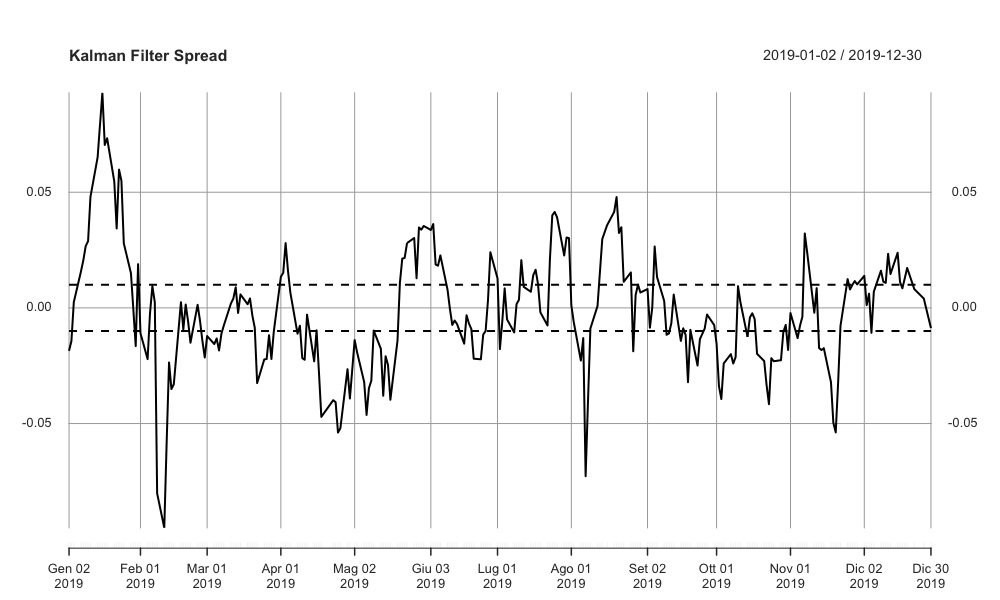
\includegraphics[width=.8\textwidth]{ucg_bpe_kfspread.png}%
		}
		
		\subfigure[Cointegration Spread]{%
			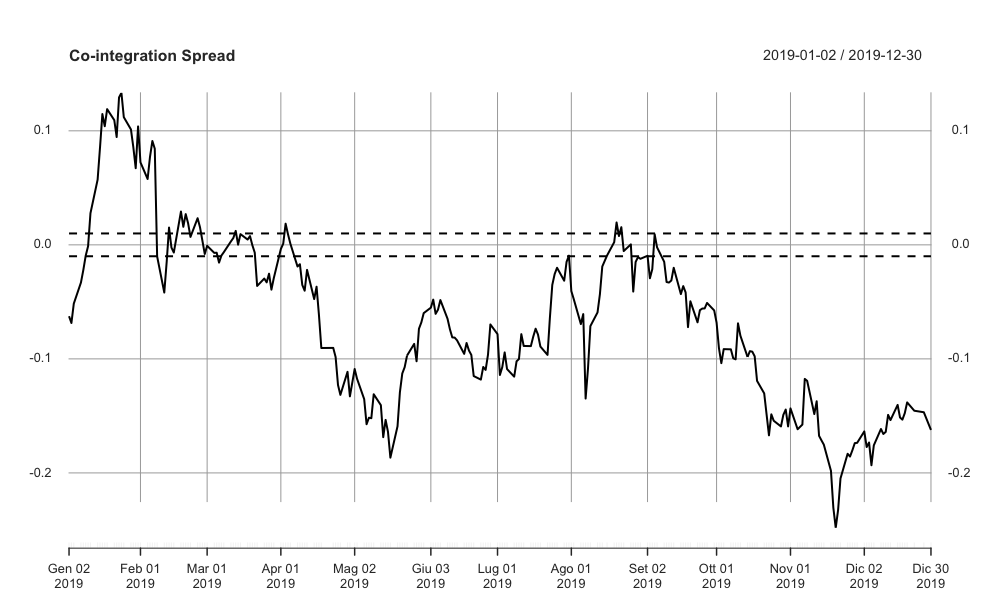
\includegraphics[width=.8\textwidth]{ucg_bpe_lsspread.png}%
		}
		\subfigure[Rolling Regression Spread]{%
			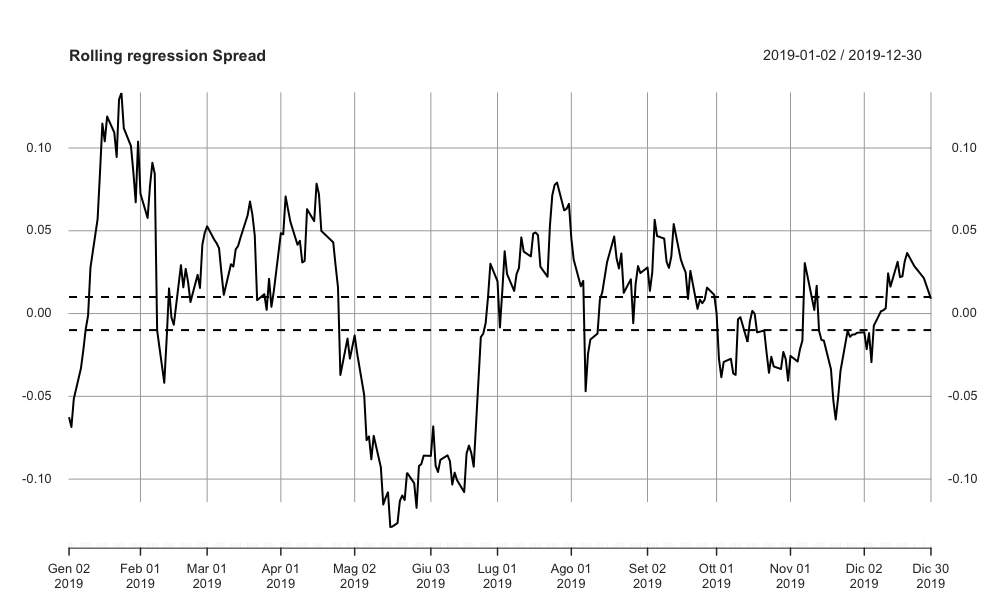
\includegraphics[width=.8\textwidth]{ucg_bpe_rlspread.png}%
		}
		\caption{\textbf{Spread per le tre metodologie,UCG.MI-BPE.MI}}
		\label{spread_ucg_bpe}
		
	\end{center}
\end{figure}


\
\\
\begin{figure}[htp]
	\begin{center}
		
		\subfigure[\textbf{$\alpha$}]{%
			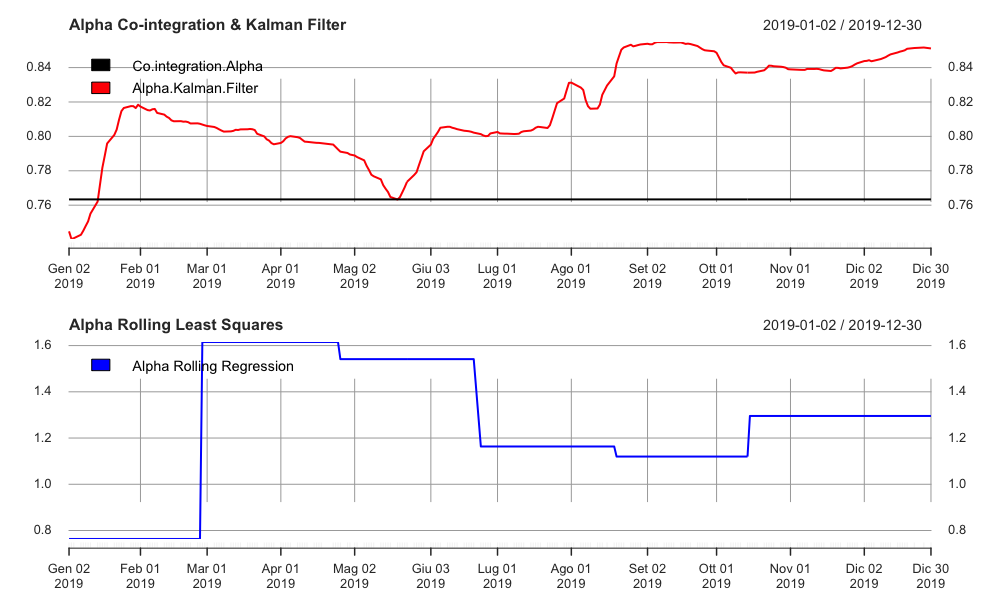
\includegraphics[width=.8\textwidth]{ucg_bpe_alpha.png}%
		}
		
		\subfigure[\textbf{$\beta$}]{%
			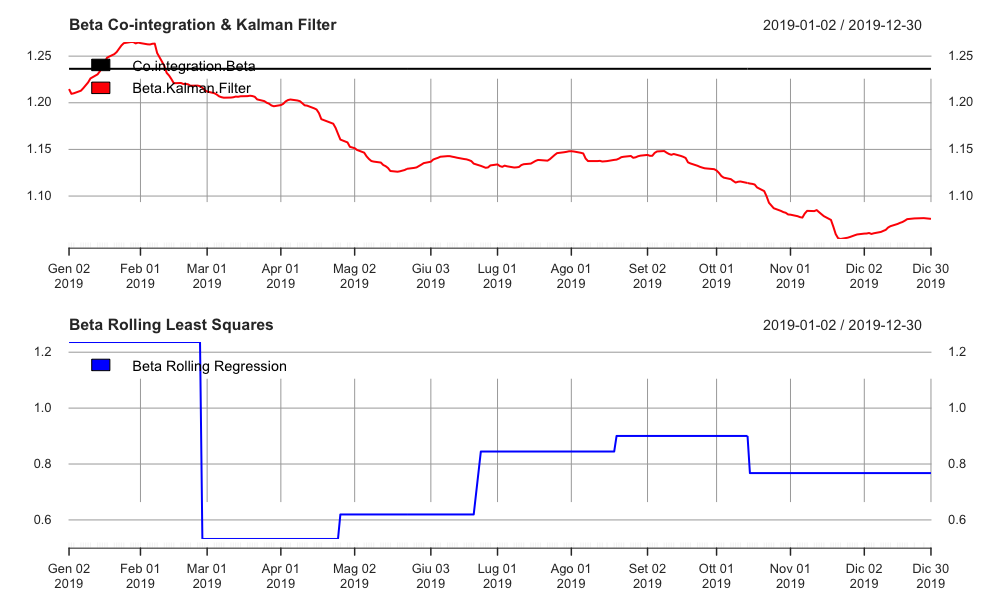
\includegraphics[width=.8\textwidth]{ucg_bpe_beta.png}%
		}
		
		\caption{\textbf{Alpha e Beta,UCG.MI-BPE.MI}}
		
	\end{center}
\end{figure}


\begin{figure}
	\centering
	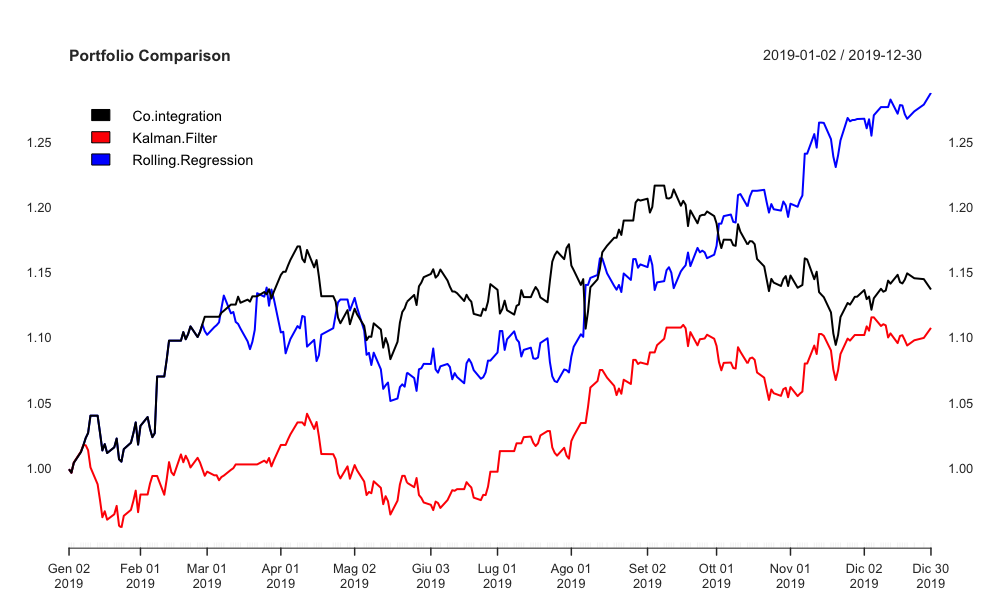
\includegraphics[scale=0.3]{ucg_bpe_portfolio.png}
	\caption{\textbf{P\&L,UCG.MI-BPE.MI}}
\end{figure}

\break

\subsection*{ Banca Mediolanum S.p.A. - Banca Generali S.p.A.}

La terza coppia considerata (in ordine di correlazione) è formata dalle multinazionali \textbf{Banca Mediolanum S.p.A.} e  \textbf{Banca Generali S.p.A.}, entrambe operanti nel settore dei servizi finanziari.

\begin{center}
	\captionof{table}{Analisi dei processi,BMED.MI-BGN.MI}\label{stazionarietà_bmed_bgn}
	\begin{tabular}{ p{2cm}p{3cm}p{1cm}p{2cm}p{1cm}}
		\hline
		Processo & Metodologia & ADF Statistic & p-value & RMSE \\
		\hline
		$S_1$ & Cointegrazione & -0.54 &  0.97 & 0.110  \\
		$S_2$ & Kalman Filter & -3.60 &  0.03 &  0.012 \\
		$S_3$ & Rolling Regression & -0.79 & 0.96 & 0.098 \\
		\hline
	\end{tabular}
\end{center}
\
\\
Dai risultati delle statistiche test in tabella \ref{stazionarietà_bmed_bgn} è evidente come per i metodi di Cointegrazione e Rolling Regression, il vettore cointegrante $\hat{\beta}$ non riesca a rendere stazionario il \textit{trading period}.
Chiaramente visibile anche in figura \ref{spread_bmed_bgn}, è la rottura della relazione di cointegrazione tra le serie storiche di Banca Mediolanum e Banca Generali.
Ciò che si evince da questa analisi è come l'ipotesi di persistenza della stazionarietà del processo ottenuto come combinazione di vettori statici sia poco plausibile nel contesto dinamico delle serie di titoli finanziari, break strutturali sono presenti anche in contesti simili del mercato finanziario, evidenziando la rischiosità della strategia.
\\
La Tabella \ref{performance_bmed_bgn} mostra le performance per i tre modelli.
\\
La media dello Sharpe Ratio per i tre modelli, del 12\% , ci indica che per la coppia considerata, nel \textit{trading period}, il rendimento del portafoglio in rapporto al rischio è stato basso.
Sebbene il metodo Rolling Regression ottenga la miglior performance in termini di rendimento, il range di variazione delle perdite misurato dal Max Drawdown è del 15\% del valore del portafoglio.
In figura \ref{portfolio_bmed_bgn} è visibile come a partire da Novembre 2019 la shock della rottura del legame di cointegrazione tra Banca Mediolanum e Banca Generali porti questo tipo di strategia ad essere perdente per tutte le metodologie considerate.

% PERFORMANCE
\begin{center}
	\captionof{table}{Analisi trading performance,BMED.MI-BGN.MI}
	\label{performance_bmed_bgn}
	\begin{tabular}{ p{3cm}p{2cm}p{1cm}p{1cm}p{1cm}p{1cm}}
		\hline
		Metodologia  & Sharpe Ratio & MDD & Returns & VaR & ES\\
		\hline
		Cointegrazione & 0.12 &  0.17 & 0.007& 0.25 & 0.29\\
		Kalman Filter & 0.14 &   0.08 & -0.006 & 0.24 & 0.27 \\
		Rolling Regression & 0.17 &  0.15 &  0.013 & 0.25 & 0.28 \\
		\hline
	\end{tabular}
\end{center}
\
\\\\\\\\\\\\\\
\begin{center}
	\begin{tabular}{@{}llll@{}}
		\toprule
	From       & To         & Depth   & Length \\ \midrule
	2019-01-09 & 2019-02-11 & -0.0231 & 24     \\
	2019-02-28 & 2019-05-13 & -0.0445 & 50     \\
	2019-05-23 & 2019-06-12 & -0.0237 & 15     \\
	2019-08-13 & 2019-08-16 & -0.0139 & 3      \\
	\rowcolor[HTML]{FFCCC9} 
	2019-09-10 & NA         & -0.1753 & 78     \\ \bottomrule
	\end{tabular}
	\captionof{table}{Analisi Drawdowns,Cointegrazione}\label{drawdowns_bmed_bgn_coint}
\end{center}
\
\\
\begin{center}
	\begin{tabular}{@{}llll@{}}
		\toprule
		From       & To         & Depth   & Length \\ \midrule
		2019-01-10 & 2019-04-01 & -0.0622 & 58     \\
		\rowcolor[HTML]{FFCCC9} 
		2019-04-15 & 2019-08-08 & -0.0741 & 81     \\
		2019-08-16 & 2019-08-27 & -0.0179 & 8      \\
		2019-09-18 & 2019-12-05 & -0.0518 & 57     \\
		2019-12-09 & NA         & -0.0193 & 14     \\ \bottomrule
	\end{tabular}
	\captionof{table}{Analisi Drawdowns,Kalman Filter}\label{drawdowns_bmed_bgn_kf}
\end{center}

\
\\
\begin{center}
	\begin{tabular}{@{}llll@{}}
		\toprule
	From       & To         & Depth   & Length \\ \midrule
	2019-01-09 & 2019-02-11 & -0.0231 & 24     \\
	2019-02-28 & 2019-04-24 & -0.0295 & 38     \\
	2019-04-30 & 2019-08-09 & -0.0531 & 73     \\
	2019-08-13 & 2019-08-16 & -0.0142 & 3      \\ 
	\rowcolor[HTML]{FFCCC9} 
	2019-10-08 & NA         & -0.1534 & 58    \\ \bottomrule
	\end{tabular}
	\captionof{table}{Analisi Drawdowns,Rolling Regression}\label{drawdowns_bmed_bgn_rl}
\end{center}
\
Dalle tabelle \ref{drawdowns_bmed_bgn_coint}, \ref{drawdowns_bmed_bgn_kf} e \ref{drawdowns_bmed_bgn_rl} si evince che il modello Kalman Filter subisce periodi di drawdown più lunghi ma con perdite minori rispetto agli altri due modelli.
Dalla rottura del legame di cointegrazione il metodo di Cointegrazione ha un 17\% di drawdown rispetto al valore del portafoglio, per un periodo di 78 giorni consecutivi.
La Rolling Regression un 15\% di drawdown per un periodo di 58 giorni consecutivi.
\begin{figure}[htp]
	\begin{center}
		
		\subfigure[Kalman Filter spread]{%
			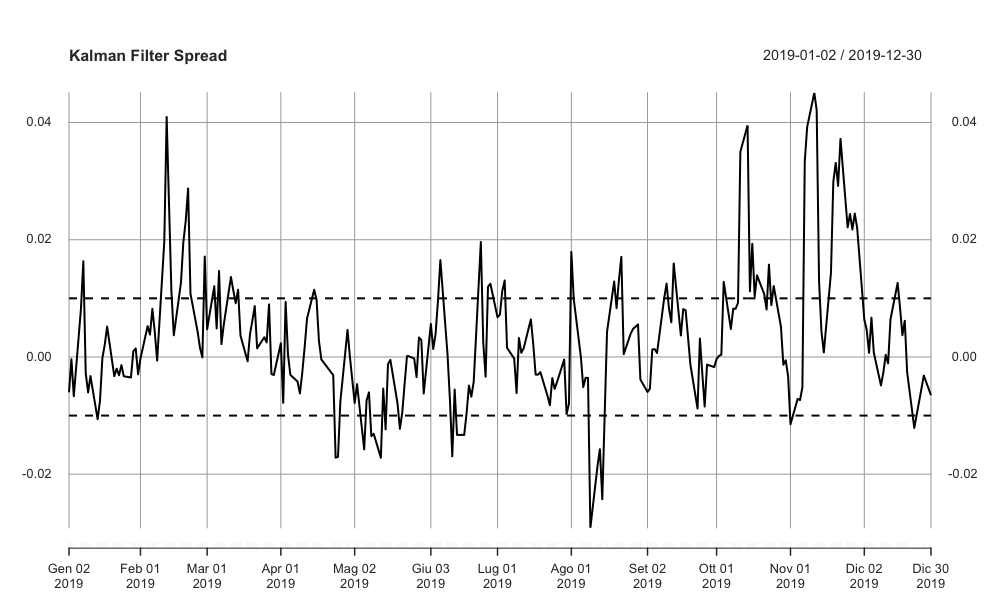
\includegraphics[width=.8\textwidth]{bmed_bgn_kfspread.png}%
		}
		
		\subfigure[Cointegration Spread]{%
			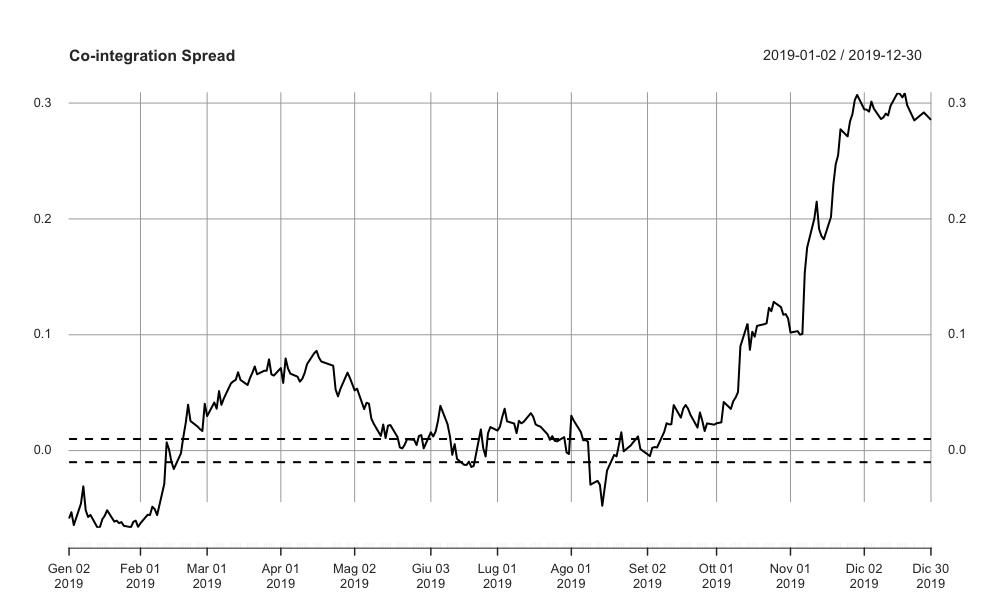
\includegraphics[width=.8\textwidth]{bmed_bgn_lsspread.png}%
		}
		\subfigure[Rolling Regression Spread]{%
			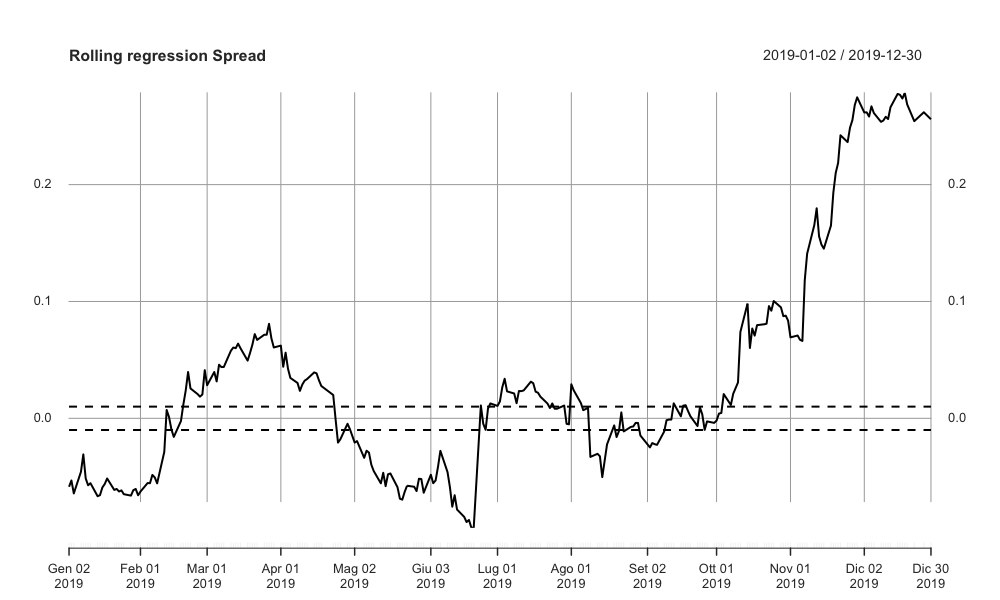
\includegraphics[width=.8\textwidth]{bmed_bgn_rlspread.png}%
		}
		\caption{\textbf{Spread per le tre metodologie,BMED.MI-BGN.MI}}
		\label{spread_bmed_bgn}
	\end{center}
\end{figure}


\
\\
\begin{figure}[htp]
	\begin{center}
		
		\subfigure[\textbf{$\alpha$}]{%
			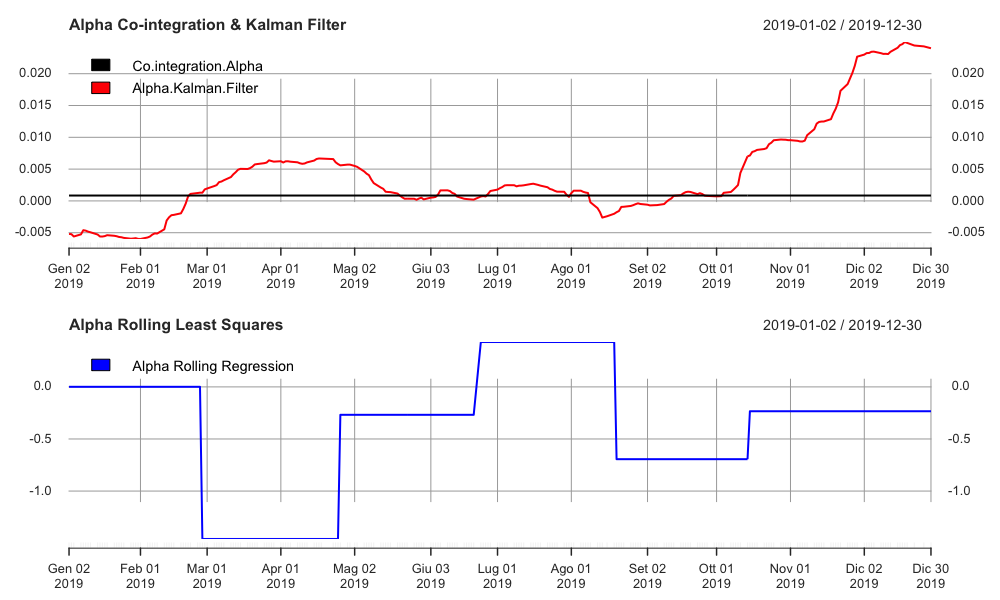
\includegraphics[width=.8\textwidth]{bmed_bgn_alpha.png}%
		}
		
		\subfigure[\textbf{$\beta$}]{%
			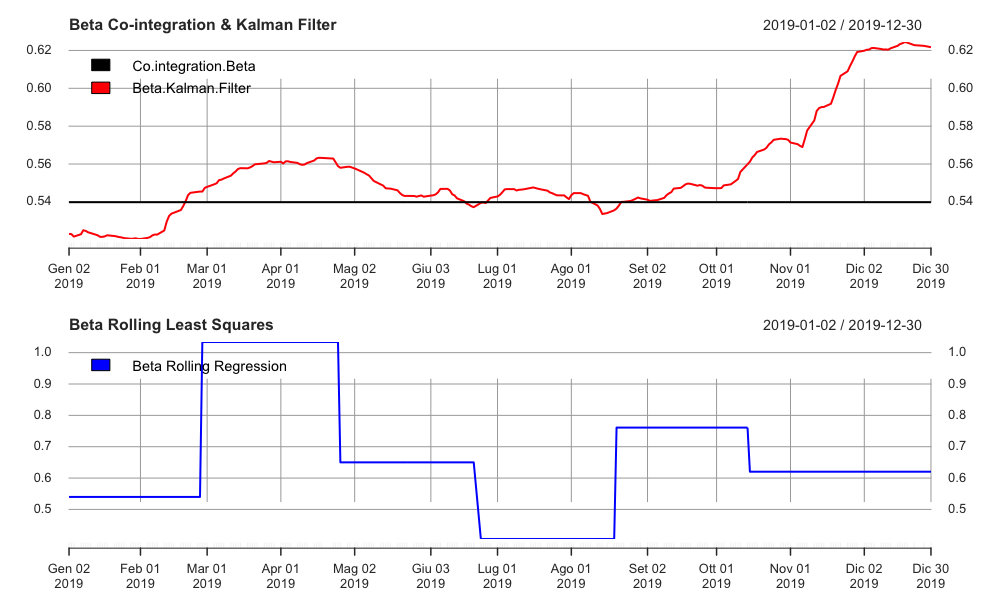
\includegraphics[width=.8\textwidth]{bmed_bgn_beta.png}%
		}
		
		\caption{\textbf{Alpha e Beta,BMED.MI-BGN.MI}}
		
	\end{center}
\end{figure}


\begin{figure}
	\centering
	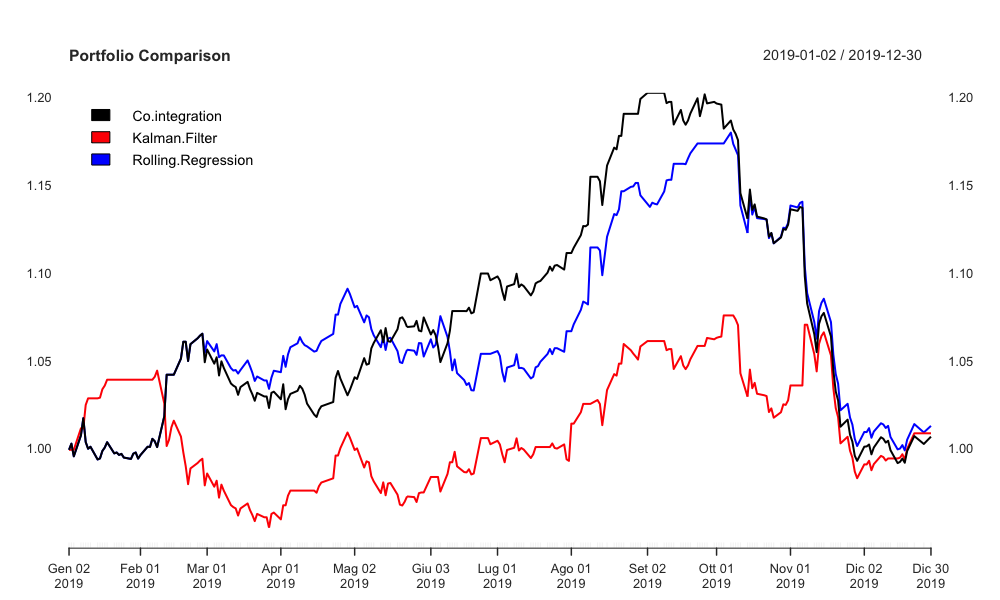
\includegraphics[scale=0.3]{bmed_bgn_portfolio.png}
	\caption{\textbf{P\&L,BMED.MI-BGN.MI}}
	\label{portfolio_bmed_bgn}
\end{figure}

\break

\subsection*{Banca Mediolanum S.p.A. - Azimut Holding S.p.A. }

La quarta coppia considerata è formata dalle multinazionali \textbf{Banca Mediolanum S.p.A.} e  \textbf{Azimut Holding S.p.A.}, entrambe operanti nel settore dei servizi finanziario-assicurativi.

\begin{center}
	\captionof{table}{Analisi dei processi, BMED.MI-AZM.MI}\label{stazionarietà_bmed_azm}
	\begin{tabular}{ p{2cm}p{3cm}p{1cm}p{2cm}p{1cm}}
	\hline
	Processo & Metodologia & ADF Statistic & p-value & RMSE \\
	\hline
	$S_1$ & Cointegrazione &-0.69 &  0.96 & 0.11 \\
	$S_2$ & Kalman Filter & -4.15 &  0.01 & 0.011 \\
	$S_3$ & Rolling Regression & -1.99 & 0.57 & 0.04 \\
	\hline
	\end{tabular}
\end{center}
\
\\
Il caso qui presentato è forse quello più interessante rispetto ai tre precedentemente presentati.
Dalla tabella \ref{stazionarietà_bmed_azm} i valore dell'ADF test ci portano ad accettare l'ipotesi di non stazionarietà per i processi $S_1, S_3$.
Il modello Kalman Filter ha il minor errore quadratico medio, confermando come questo approccio abbia sostanzialmente minor distorsione rispetto agli altri metodi considerati e che la stima del vettore cointegrante riesca a rendere stazionaria la combinazione lineare dei due titoli nel \textit{trading period}
\\
Come nel caso riportato precedentemente in figura \ref{spread_bmed_azm} è visibile come per l'approccio classico di cointegrazione lo spread diverga dal suo valore medio senza farne ritorno per 1/3 del \textit{trading period}. Periodo che coincide con la fase di drawdown più lunga della performance.
\\
In tabella \ref{performance_bmed_azm} i risultati ci mostrano una performance superiore per il Kalman Filter, sia in termini di rendimento che in termini di gestione del rischio.
La stazionarietà del processo $S_2$ rende il portafoglio costruito meno soggetto a variazioni estreme nelle perdite. Riassumendo anche i casi precedemente illustrati, sembrerebbe che le stime mobili dei vettori cointegranti $\hat{\alpha}$ e $\hat{\beta}$ riducano la variabilità del processo $S_2$, ciò si riflette, non tanto in una maggior profittabilità del portafoglio quanto piuttosto in riduzione dei rischi legati ai cambiamenti di regime o altri fattori che possono minare la stabilità del vettore.


% PERFORMANCE
\begin{center}
	\captionof{table}{Analisitrading performance,BMED.MI-AZM.MI}\label{performance_bmed_azm}
	\begin{tabular}{ p{3cm}p{2cm}p{1cm}p{1cm}p{1cm}p{1cm}}
		\hline
		Metodologia  & Sharpe Ratio & MDD & Returns & VaR & ES\\
		\hline
		Cointegrazione & -0.79 & 0.18 & -0.08 &  0.26 & 0.30\\
		Kalman Filter &  0.72 & 0.04 & 0.06 & 0.06 & 0.23  \\
		Rolling Regression & -1.00 & 0.13 & -0.10 & 0.24 & 0.28\\
		\hline
	\end{tabular}
\end{center}
\
\\\\\\\\\\\\\\
\begin{center}
	\begin{tabular}{@{}llll@{}}
	\toprule
	From       & To         & Depth   & Length \\ \midrule
	2019-01-15 & 2019-01-28 & -0.0266 & 10     \\
	2019-01-31 & 2019-02-06 & -0.0111 & 5      \\
	2019-02-12 & 2019-05-06 & -0.0482 & 57     \\
	2019-06-26 & 2019-08-09 & -0.0317 & 33     \\
	\rowcolor[HTML]{FFCCC9} 
	2019-08-12 & NA         & -0.1899 & 98     \\ \bottomrule
	\end{tabular}
	\captionof{table}{Analisi Drawdowns,Cointegrazione}\label{drawdowns_bmed_azm_coint}
\end{center}
\
\\
\begin{center}
	\begin{tabular}{@{}llll@{}}
	\toprule
	From       & To         & Depth   & Length \\ \midrule
	2019-01-28 & 2019-04-05 & -0.0454 & 50     \\
	2019-06-14 & 2019-06-25 & -0.0161 & 8      \\
	2019-06-26 & 2019-08-09 & -0.0249 & 33     \\
	\rowcolor[HTML]{FFCCC9} 
	2019-08-21 & 2019-11-18 & -0.0498 & 64     \\
	2019-11-20 & NA         & -0.0421 & 27     \\ \bottomrule
	\end{tabular}
	\captionof{table}{Analisi Drawdowns,Kalman Filter}\label{drawdowns_bmed_azm_kf}
\end{center}

\
\\
\begin{center}
	\begin{tabular}{@{}llll@{}}
	\toprule
	From       & To         & Depth   & Length \\ \midrule
	2019-01-09 & 2019-01-11 & -0.0056 & 3      \\
	2019-01-15 & 2019-01-28 & -0.0266 & 10     \\
	2019-01-31 & 2019-02-06 & -0.0111 & 5      \\
	\rowcolor[HTML]{FFCCC9} 
	2019-02-12 & NA         & -0.1371 & 224    \\ \bottomrule
	\end{tabular}
	\captionof{table}{Analisi Drawdowns,Rolling Regression}\label{drawdowns_bmed_azm_rl}
\end{center}
\
L'analisi dei drawdown per la coppia BMED.MI - AZM.MI evidenzia che il metodo di Rolling Regression registra una performance in ribasso per quasi tutto il \textit{trading period}, con 224 giorni consecutivi di perdite da Febbraio 2019.


\begin{figure}[htp]
	\begin{center}
		
		\subfigure[Kalman Filter spread]{%
			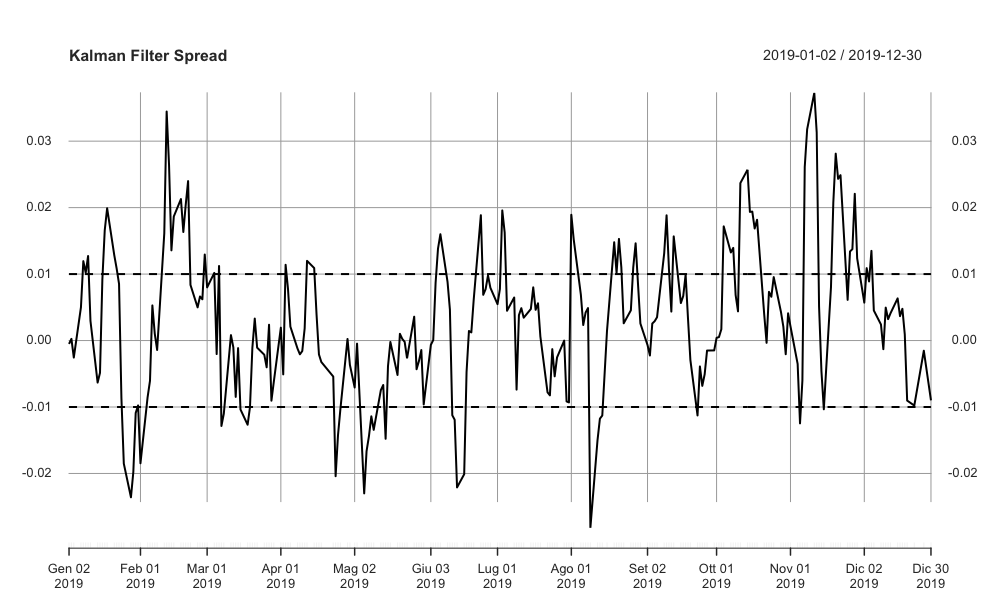
\includegraphics[width=.8\textwidth]{bmed_azm_kfspread.png}%
		}
		
		\subfigure[Cointegration Spread]{%
			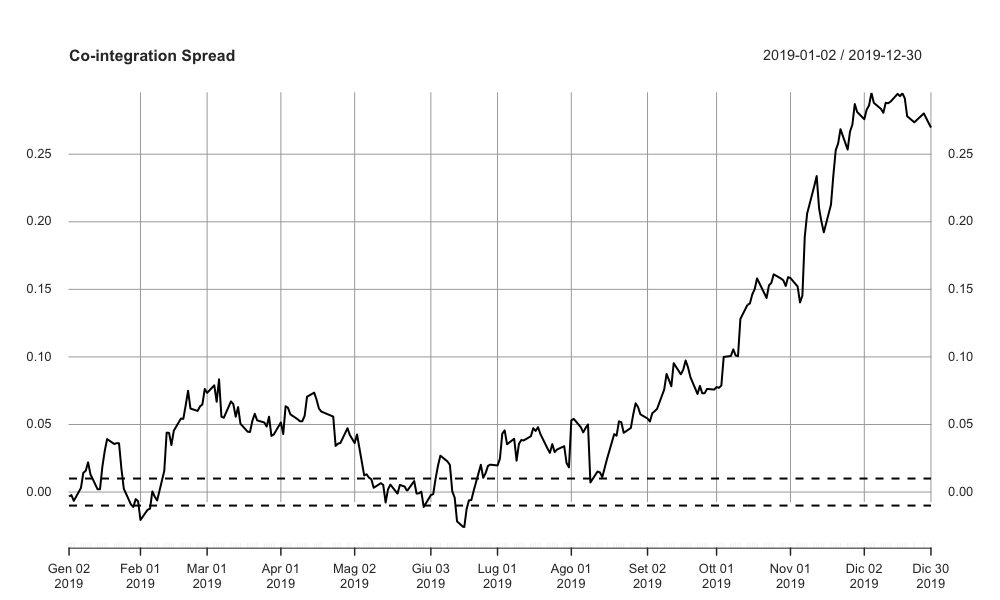
\includegraphics[width=.8\textwidth]{bmed_azm_lspread.png}%
		}
		\subfigure[Rolling Regression Spread]{%
			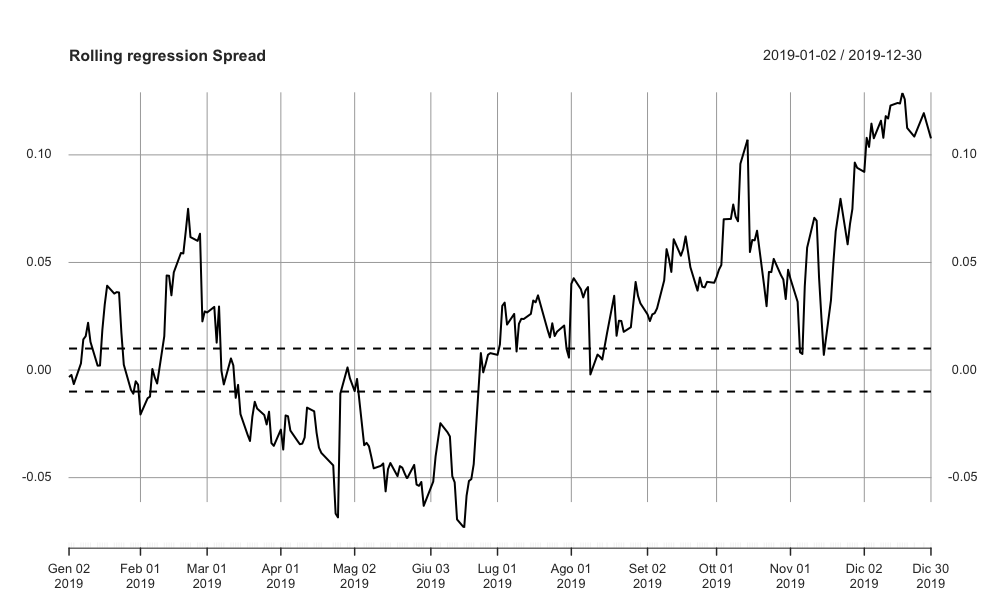
\includegraphics[width=.8\textwidth]{bmed_azm_rlspread.png}%
		}
		\caption{\textbf{Spread per le tre metodologie,BMED.MI-AZM.MI}}
		\label{spread_bmed_azm}
	\end{center}
\end{figure}


\
\\
\begin{figure}[htp]
	\begin{center}
		
		\subfigure[\textbf{$\alpha$}]{%
			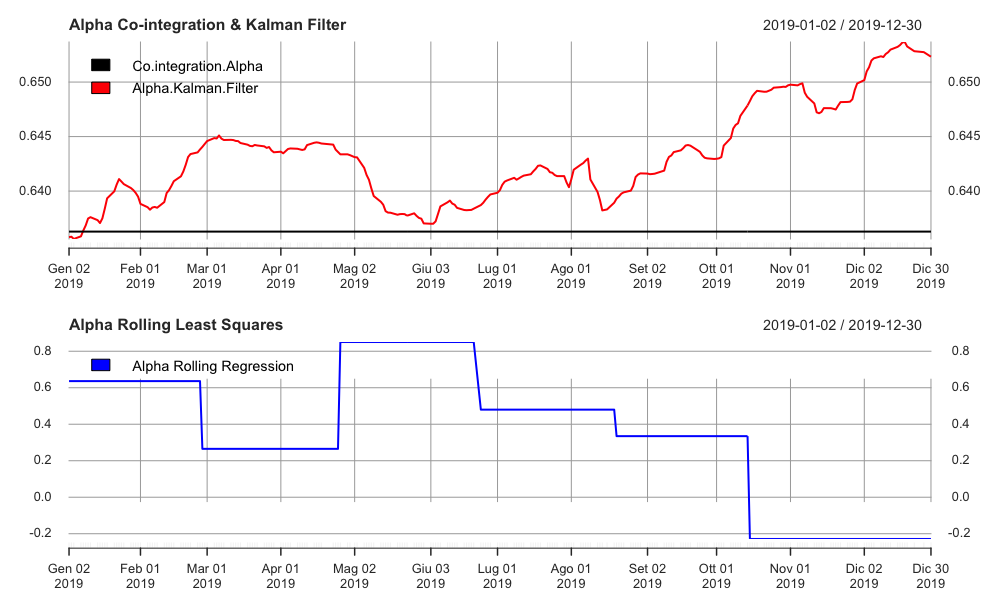
\includegraphics[width=.8\textwidth]{bmed_azm_alpha.png}%
		}
		
		\subfigure[\textbf{$\beta$}]{%
			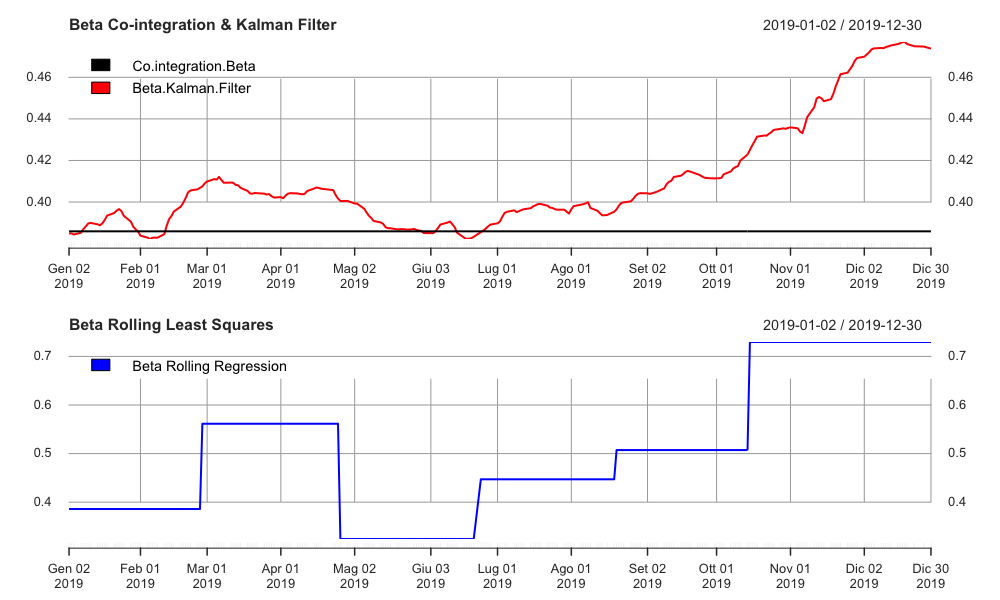
\includegraphics[width=.8\textwidth]{bmed_azm_beta.png}%
		}
		
		\caption{\textbf{Alpha e Beta,BMED.MI-AZM.MI}}
		
	\end{center}
\end{figure}


\begin{figure}
	\centering
	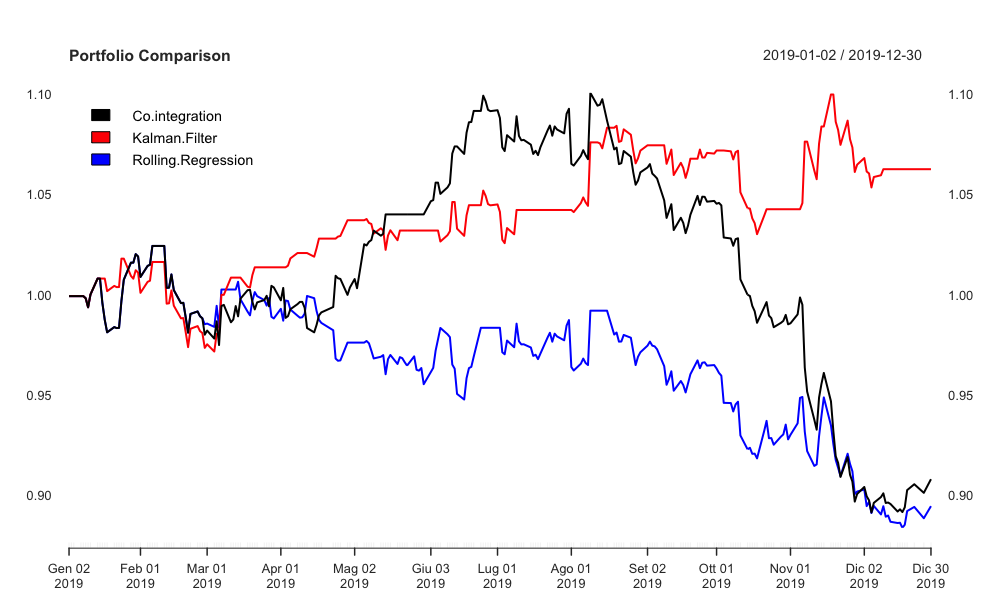
\includegraphics[scale=0.3]{bmed_azm_portfolio.png}
	\caption{\textbf{P\&L,BMED.MI-AZM.MI}}
\end{figure}

\break

\section*{Conclusioni}
\addcontentsline{toc}{section}{Conclusioni}


Alla luce del diffondersi di strategie di mercato basate sull’econometria applicata e su particolari relazioni tra i prezzi di asset finanziari, questo lavoro ha voluto fornire un contributo analitico sull'applicabilità di alcuni di questi modelli. Il nostro studio si è focalizzato sul ruolo della cointegrazione nello sviluppo di una strategia di \textit{Pair Trading}.
Nel corso della trattazione è stato costruito un modello operativo basato su strumenti e principi di econometria finanziaria, questo modello è stato poi messo alla prova valutandone aspetti che vanno oltre la capacità di ottenere risultati positivi.
Per la costruzione e l'analisi del modello operativo è stato scelto di utilizzare quotazioni reali dei titoli dell'indice della borsa italiana, il  FTSE MiB.
Su questi sono stati implementati test econometrici che ci hanno consentito di individuare la presenza di relazioni di cointegrazione nel paniere dei 40 titoli scelti.
Stimato il vettore di cointegrazione e quindi ottenuto il processo stocastico dalla combinazione dei titoli, abbiamo illustrato l'applicabilità della strategia procedendo con un Back Testing della stessa. La valutazione ha condotto ad evidenze interessanti. 
\\
Sulla persistenza delle relazioni di cointegrazione, appaiono ragionevoli,per il mercato italiano, le evidenze riscontrate da Clegg (2014) sui costituenti del S\&P 500.
La \textit{"proprietà"} che identifica la cointegrazione come relazione di lungo termine tra due serie storiche è quantomeno soggetta al beneficio del dubbio.
In un ottica statistica, riportata su strategie di investimento, sostenere che questa sarà presente in un arco temporale abbastanza lungo da ottenere profitti, sottopone l'investitore a un rischio notevole,considerando la mutevolezza dei mercati finanziari.
In tal senso è risultata evidente una caratteristica di non poco conto.
I profitti maggiori per le coppie considerate sono stati ottenuti nei casi in cui il processo manteneva la sua caratteristica principale di \textit{mean-reversion}. Ciò è particolarmente evidente nel primo caso e nel secondo caso illustrato in questa trattazione.
Laddove il processo rimane stazionario, la profittabilità della strategia è quantomeno mitigata dal minor rischio corso durante l'investimento.
L'utilizzo di un modello nello spazio degli stati contrapposto a metodi più \textit{"classici"} ha evidenziato come  una stima più robusta dei vettori di cointegrazione ( o per meglio dire \textit{aggiornata}) giochi a beneficio di questa caratteristica.
Nonostante la sua applicazione sia avvenuta in un contesto privo di frizioni di mercato, la strategia è stata in grado di ottenere rendimenti positivi laddove si presentavano le condizioni ideali.
A tal scopo, sottolineiamo che la scelta di operare in condizioni semplificate mirava allo scopo di questo lavoro; l'analisi dei metodi di cointegrazione nelle serie storiche.
L'analisi proposta in questo lavoro , di fatti, deficita di una componente fondamentale da considerare in una strategia di investimento: il costo di investire.
Nonostante l’utilizzo di strumenti econometrici possa garantire una credibilità più consistente rispetto a strategie basate sul sentiment o su altri fattori scarsamente teorizzabili (o se teorizzabili più semplicistici), un money management inadatto o una scarsa considerazione di fattori quali commissioni,slippage,costi overnight, possono azzerare il vantaggio statistico derivante da queste metodologie.
Lo studio di questo tipo di strategie non è esente da questi aspetti come da quelli di miglioramento degli strumenti econometrici utilizzati. Una comparazione di differenti modelli operativi al variare dei parametri (thresholds, periodo di operatività,capitale investito) risulta ancora più necessaria dalle conclusioni di questo lavoro.
Pertanto il risultato fondamentale è  dato dalla completa teorizzazione del modello e dall’identificazione di alcuni punti critici che, alla luce dello stato dell’arte di alcune tecniche di stima, possono costituire il punto di partenza per una sua evoluzione.




\break

\appendix
\section*{Appendice Teorica}
\addcontentsline{toc}{section}{Appendice Teorica}
\renewcommand{\thesubsection}{\Alph{subsection}}

\subsection{Processi Stocastici}
\subsubsection*{Processo stocastico discreto}
Dato uno spazio di probabilità $(\Omega,\mathcal{A},P)$, un processo stocastico discreto è una successione di variabili aleatorie definite sullo spazio di probabilità $\Omega$:
\begin{equation}
	(X_n)_{n \ge0}
\end{equation}
\
dove 
\begin{itemize}
	\item $\mathcal{A}$ è una $\sigma$-algebra di $\Omega$
	\item P è una misura di probabilità definita su ($\Omega$,$\mathcal{A}$)
\end{itemize}
\
Il termine "discreto" si riferisce al fatto che il numero di istanti, nell'evoluzione temporale del processo, è finito.
\subsubsection*{Stazionarietà di un processo stocastico}

Un processo stocastico $\mathbf{\epsilon_t}$ è detto debolmente stazionario se il suo momento primo e il suo momento secondo sono costanti nel tempo. Intuitivamente, ciò ci dice che la struttura probabilistica di un processo stazionario non cambia nel tempo.
In altre parole, $\epsilon_t$ è stazionario se 

\
\begin{itemize}
	\item $\E[\epsilon_t]= \mu \qquad \forall \; t \in T $ 
	\item $V[\epsilon_t] = \sigma^2 \qquad \forall \; t \in T$ 
	\item $Cov[\epsilon_t,\epsilon_{t-k}]=\gamma_k \qquad \forall \; t \in T \qquad k=  0, \pm 1, \pm 2, ...$
\end{itemize}
\
\\
La prima condizione indica che tutti i membri di un processo stocastico debolmente stazionario hanno media costante. La seconda condizione assicura che anche il suo momento secondo sia costante.
Un processo $\epsilon_t$ stazionario è possibile indicarlo come $\mathbf{\epsilon_t \sim I(0)}$.
\\
Le condizioni definite fin qui sono fondamentali nella costruzione di una strategia di trading basata sulla cointegrazione, in quanto un serie storica generata da un processo stocastico stazione deve fluttuare intorno a un valore medio costante e non deve avere un trend.
L'oscillazione intorno a un valore medio, o fenomeno di \textit{mean reversion} è  infatti l'elemento che permette di generare segnali quando lo \textit{spread} di cointegrazione si allontana dal suo valore medio.
Quando le caratteristiche del processo stocastico cambiano nel tempo si può parlare di processo non stazionario. All’interno della classe dei processi non stazionari e integrati è presente un tipo di processo autoregressivo di grande utilità nella nostra trattazione, il processo \textit{random walk}.

\subsubsection*{Processi a radice unitaria}
Definiamo il concetto di \textit{integrazione} di una serie storica.
Un processo I(1) (integrato di ordine 1) è un processo non stazionario di cui è stazionaria la differenza prima. Più in generale, si definisce come processo I(d) un processo la cui differenza \textit{d-esima} è stazionaria.
Il più semplice esempio di processo lineare omogeneo non stazionario e integrato di ordine 1 è il cosiddetto \textit{random walk} o \textit{passeggiata casuale}.

\subsubsection*{Random Walk}

Un processo \textit{Random Walk} è definito come

\begin{equation}
	S_t = \epsilon_1 + \epsilon_2 + ... + \epsilon_t = S_{t-1} + \epsilon_t
\end{equation}
\
Dove $S_0= 0$ e $\epsilon_t \sim WN(0,\sigma_{\epsilon}^2)$.
\\
Ad ogni istante \textit{t} la media del processo è pari a 0 ma la varianza dipende dal tempo. 
\\\\
Più formalmente

\begin{itemize}
	\item $\E[S_t]=0$
	\item $V[S_t]= t\sigma_{\epsilon}^2$
\end{itemize}
\
Tale processo, come già precisato, è non stazionario. Infatti, la varianza di un processo random walk cresce linearmente in funzione del tempo, incrementando all’infinito.
Seppur non stazionario nella sua natura, un processo random walk è stazionario nelle prime differenze o più specificamente
\begin{equation}
	\Delta S_t = S_t - S_{t-1} = \epsilon_t
\end{equation}
\
La prima differenza di un processo \textit{random walk} è un processo \textit{white noise}.
Un processo random walk è per definizione una martingala, cioè è  tale che il valore assunto domani da una variabile aletoria sia pari al valore di oggi più un valore imprevedibile.



\subsection{Test di radice unitaria}

I processi integrati, così come visti finora, hanno delle caratteristiche che li
rendono molto interessanti, sia da un punto di vista formale (perché rappresentano un esempio di processi non stazionari), che da un punto di vista
pratico (perché le loro realizzazioni somigliano in modo spiccato alle serie
storiche che siamo abituati ad incontrare in macroeconomia).
La  stazionarietà di un fenomeno come abbiamo visto presenta delle caratteristiche ben marcate (prima su tutte l'oscillazione del processo intorno a una media costante), si rende però necessario individuare delle regole di decisione che permettano di specificare se un processo è stazionario o non. Regole di decisione di questo tipo sono note come \textbf{test di radice unitaria}.
\subsubsection*{Dickey Fuller Test}

Consideriamo un progresso autogressivo del primo ordine,AR(1) del tipo

\begin{equation}
	y_t = \phi y_{t-1} + u_t
\end{equation}
\
Se per definizione vale la relazione
\begin{equation}
	\Delta y_t =\rho y_{t-1} + u_t
\end{equation}
\
dove $u_t$ è un \textit{white noise} e $\rho= \phi - 1$ il sistema di ipotesi da saggiare è del tipo

\begin{equation}
	\begin{cases}
		H_0: \rho = 0 \\
		H_1 : \rho < 0
	\end{cases}
\end{equation}
\
Ossia l'ipotesi nulla di non stazionarietà(se $\rho= 0$ allora $\phi = 1$) contro l'ipotesi alternativa di stazionarietà($\rho < 0 $ e quindi $\phi < 1 $).
Il \textbf{Test di Dickey Fuller} , ossia un test di radice unitaria,si potrebbe vedere come un test \textit{t}  di azzeramento del parametro $\rho$ ossia un test basato sulla statistica 

\begin{equation}
	t_p = \frac{\hat{\rho}}{std(\hat{\rho})}
\end{equation}
\
dove le stime di $\rho$ indicano le stime OLS.
\\
Tale statistica segue un'apposita distribuzione tabulata per primo da Fuller.
Il fatto che l’ipotesi di non stazionarietà implichi $\phi=1$ è la ragione per cui questo test viene spesso chiamato test unit root (radice unitaria).
Generalmente per la scelta del livello di significatività della statistica test viene scelto un valore pari a $\alpha=0.05$, per cui in questo caso si possono verificare le seguenti situazioni:

\begin{enumerate}
	\item Se il \textit{p-value} $> \alpha$ si accetta l'ipotesi nulla di non-stazionarietà del processo, con un livello di confidenza del 95\&%
	\item Se il \textit{p-value} $< \alpha$ l'ipotesi nulla viene rifiutata, quindi la serie è stazionaria.
\end{enumerate}


\subsubsection*{Augmented Dickey Fuller Test}

Consideriamo il processo $y_t$ caratterizzato da una struttura ARMA. Per verificare l'esistenza di radici unitaria nella parte AR(p) testiamo, sotto l'ipotesi nulla che il processo abbia una radice unitaria, il seguente sistema di ipotesi
\begin{equation}
	\begin{cases}
		H_0 : \beta = 1 \\
		H_1 : \beta < 1
	\end{cases}
\end{equation}
attraverso una regressione del tipo

\begin{equation}
	y_t = c_t + \beta y_{t-1}+ \sum_{i=1}^{p-1} \phi_i \Delta y_{t-1} + \epsilon_t
\end{equation}
\
il \textit{t} ratio di $\hat{\beta} - 1$, per saggiare il sistema di ipotesi sopra definito è

\begin{equation}
	ADFtest = \frac{\hat{\beta}-1}{std(\hat{\beta})}
\end{equation}
\
\\
La statistica test prende il nome di  \textit{Augmented Dickey Fuller Test}, dove $\hat{\beta}$ indica la stima di $\beta$ ottenuta con il metodo dei minimi quadrati.
Se il valore calcolato della statistica test è minore di un valore critico, allora l'ipotesi nulla di non stazionarietà (presenza di una radice unitaria) è rifiutata.

\subsubsection*{Distribuzione della statistica Test}

I quantili di questa distribuzione vanno calcolati attraverso
simulazioni numeriche, ed i primi che l’hanno fatto sono stati Dickey e Fuller
nel 1976, ragion per cui talvolta questa distribuzione viene chiamata distribuzione DF, o Dickey-Fuller. Per lo stesso motivo, anche il test è noto come test
DF. 

\break

\appendix
\section*{Implementazione in R}
\addcontentsline{toc}{section}{Implementazione in R}

\subsection*{Analisi di cointegrazione}
\begin{lstlisting}[language=R]
find_cointegrated_pairs <- function(dataset,
method,
split_date,
plot=FALSE)
{
	library(tidyverse)
	library(tseries)
	library(quantmod)
	library(readxl)
	library(urca)
	

	test_df <- read.csv(dataset)
	cost <- read_excel('ftsemib_cost.xlsx')
	
	# converto in xts
	real <- xts(test_df[,-ncol(test_df)],
	order.by = as.POSIXct(test_df[,ncol(test_df)]))
	
	# escludo il 2020
	if(cut_2020){
		real <- real['::2020-01-01']
	}
	else{NULL}
	
	
	########################  SE METODO LOG
	if(method=='log')
	{
		for(i in 1:ncol(real))
		{
			real[,i] <- log(real[,i])
		}
		real <- na.omit(real)
		print('Cointegrazione calcolata sui log-prezzi')
		print("___________________________________________")
	}
	else{
		NULL
	}
	
	######## 
	########
	# SOLO TRAIN
	train_real <- real[paste0('::',split_date)]
	
	# Test per il plot
	test_real <- real[paste0(split_date,'::')]
	
	print(paste('Verifico la  cointegrazione nel periodo:',
	head(index(train_real),1),
	'-',tail(index(train_real),1)))
	print('___________________________________________')
	
	# nomi dei tickers
	tickers <- colnames(train_real)
	
	y <-NULL
	x <-NULL
	correlation<-NULL
	beta<-NULL
	pvalue_adftest <-NULL
	pvalue_pptest <- NULL
	adf_st <- NULL
	adf_order <- NULL
	pp_st <- NULL
	
	
	# numero di correlazioni da calcolare
	n_correlations <- (ncol(real)^2-ncol(real))/2
	print(n_correlations)
	# cosa vuoi usare?
	data <- train_real
	
	for (i in 1:length(tickers)) {
		for (j in 1:length(tickers)) {
			
			if (i>j) {
				# SINISTRA / DESTRA
				y <-c(y, tickers[i])
				x <-c(x, tickers[j])
				
				# Correlazioni sui prezzi originali
				correlation<-c(correlation, 
				cor(data[,tickers[i]], 
				data[,tickers[j]]))
				
				
				
				# regressione lineare con intercetta
				m <-lm(data[,tickers[i]] ~ data[,tickers[j]])
				
				# beta
				beta<-c(beta, as.numeric(coef(m)[2]))
				
				# spread
				spread <- residuals(m)
				
				# adf test
				pvalue_adftest<-c(pvalue_adftest, 
				adf.test(spread)$p.value)
				
				adf_st <- c(adf_st,
				adf.test(spread)$statistic)
				
				adf_order <- c(adf_order,
				adf.test(spread)$parameter)
				
				# pp test
				pvalue_pptest <-c(pvalue_pptest,
				pp.test(spread)$p.value)
				
				pp_st <- c(pp_st,pp.test(spread)$statistic)
			}
		}
		
	}
	
	# risultato dell'analisi
	df<-data.frame(y, x, correlation, beta, 
	adf_st,pvalue_adftest,
	adf_order,pvalue_pptest,pp_st)
	
	# filtra per il p-value dell'adf test
	out_df <- df %>% filter(pvalue_adftest < 0.05) %>% arrange(-correlation)
	
	# aggiungi settori
	out_df$sector_leftside <- cost$Settore[match(out_df$y,cost$Ticker)]
	out_df$sector_rightside <- cost$Settore[match(out_df$x,cost$Ticker)]
	
	# filtra per settori uguali
	out_df <- out_df[which(out_df$sector_leftside==out_df$sector_rightside),]
	
	if(plot){
		f_ticker <- out_df$y[1]
		s_ticker <- out_df$x[1]
		pl <- plot(train_real[,c(f_ticker,s_ticker)],
		main=paste(f_ticker,'-',s_ticker,'Train Period'),
		legend.loc='topright')
		pl_2 <- plot(test_real[,c(f_ticker,s_ticker)],
		main=paste(f_ticker,'-',s_ticker,'Test Period'),
		col=11:12,
		legend.loc='topright')
		par(mfrow = c(2, 1))
		plot(pl)
		plot(pl_2)
	}
	
	# stampa l'output
	print(out_df)
	
	out <- list(df = df,
	out_df = out_df)
	return(out)
}

\end{lstlisting}

\subsection*{Cointegrazione}

\begin{lstlisting}
alpha_beta_LS<- function(x_train,
y_train,
method='log',
test)
{
	
	lunghezza_train <- nrow(x_train)
	
	# REGRESSIONE
	if(method=='log')
	{
		#print('Regressione effettuata sui log-prezzi')
		regression <- lm(log(y_train) ~ log(x_train))
	}
	else
	{
		regression <- lm(y_train ~ x_train)
	}
	
	##########
	########## Alpha & beta per la lunghezza del train
	alpha_train <- xts(rep(NA,lunghezza_train),
	order.by=index(x_train))
	beta_train <- xts(rep(NA,lunghezza_train),
	order.by=index(x_train))
	
	beta_train[] <- as.numeric(regression$coefficients[2])
	
	alpha_train[] <- as.numeric(regression$coefficients[1])
	
	
	
	##########
	######### Alpha & beta per la lunghezza del test
	alpha_test <- test
	beta_test <- test
	
	beta_test[] <- as.numeric(regression$coefficients[2])
	
	
	alpha_test[] <- as.numeric(regression$coefficients[1])
	
	
	# Historical standard deviation
	h_sd <- sd(regression$residuals)
	
	# OUT
	out <- list(alpha_train=alpha_train,
	beta_train=beta_train,
	alpha_test=alpha_test,
	beta_test=beta_test,
	h_sd=h_sd)
	
	return(out)
}

\end{lstlisting}

\subsection*{Kalman Filter}

\begin{lstlisting}
kalman_filter <- function(x,
y,
alpha,
beta,
method='log',
st_var=1e-5,
ob_var=1e-3,
init_var=1e-3,
smooth)
{
	library(KFAS)
	time <- nrow(x)
	
	if(method=='log'){
		x <- log(x)
		y <- log(y)
	}else{NULL}
	
	alpha <- as.numeric(alpha[1])
	beta <- as.numeric(beta[1])
	
	# init empty variables
	beta_Kalman_filtering <- alpha_Kalman_filtering <- xts(rep(NA, time), index(x))
	colnames(alpha_Kalman_filtering) <- "Alpha Kalman Filter"
	colnames(beta_Kalman_filtering) <- "Beta Kalman Filter"
	
	# Kalman parameters
	Tt <- diag(2)
	Rt <- diag(2)
	Qt <- st_var*diag(2)  # state transition variance very small
	Zt <- array(as.vector(t(cbind(1, as.matrix(x)))), dim = c(1, 2, time))  # time-varying
	Ht <- matrix(ob_var)  # observation variance
	
	a1 <- matrix(c(alpha[1], beta[1]), 2, 1) 
	P1 <- init_var*diag(2)  # variance of initial point
	P1inf <- 0*diag(2)
	
	# create Kalman model
	model <- SSModel(as.matrix(y) ~ 0 + SSMcustom(Z=Zt, 
	T=Tt, 
	R=Rt, 
	Q=Qt, 
	a1=a1, 
	P1=P1, 
	P1inf=P1inf), H=Ht)
	
	# run Kalman filtering
	out <- KFS(model)
	alpha_Kalman_filtering[] <- out$a[-1, 1]  
	beta_Kalman_filtering[] <- out$a[-1, 2]
	
	# smoothing
	L <- smooth
	alpha_Kalman_filtering[] <- stats::filter(alpha_Kalman_filtering,
	rep(1, L)/L, sides = 1)
	alpha_Kalman_filtering <- na.locf(alpha_Kalman_filtering, fromLast = TRUE)
	beta_Kalman_filtering[] <- stats::filter(beta_Kalman_filtering, 
	rep(1, L)/L, sides = 1)
	beta_Kalman_filtering <- na.locf(beta_Kalman_filtering,
	fromLast = TRUE)
	
	out  <- list(alpha=alpha_Kalman_filtering,
	beta = beta_Kalman_filtering,
	model=out)
	
	return(out)
}
\end{lstlisting}


\subsection*{Rolling Regression}

\begin{lstlisting}
rolling_2month <- function(x_train,
y_train,
x_test,
y_test)
{
	train_reg <- lm(log(y_train)~log(x_train))
	
	alpha <- train_reg$coefficients[1]
	beta <- train_reg$coefficients[2]
	
	steps <- seq(1,nrow(x_test)-40,40)
	
	alpha_ <- data.frame()
	beta_ <- data.frame()
	dates_ <- data.frame()
	for(t in steps)
	{
		# print(paste("Nel periodo",index(x_test[t]),index(x_test[t+39])))
		# Date
		dates <- paste0(index(x_test[t]),"::",index(x_test[t+39]))
		dates_ <- rbind(dates_,dates)
		# Regressione
		reg_ <- lm(log(y_test[t:(t+40)]) ~ log(x_test[t:(t+40)]))
		#print(adf.test(reg_$residuals,k=1))
		# alpha
		alpha_ <- rbind(alpha_,reg_$coefficients[1])
		# beta
		beta_ <- rbind(beta_,reg_$coefficients[2])
	}
	
	######
	
	
	beta_0 <- alpha_0 <- y_test[dates_[1,1]]
	beta_0[] <- beta
	alpha_0[] <- alpha
	
	beta_1 <- alpha_1 <- y_test[dates_[2,1]]
	beta_1[] <- beta_[1,1]
	alpha_1[] <- alpha_[1,1]
	
	beta_2 <- alpha_2 <- y_test[dates_[3,1]]
	beta_2[] <- beta_[2,1]
	alpha_2[] <- alpha_[2,1]
	
	beta_3 <- alpha_3 <- y_test[dates_[4,1]]
	beta_3[] <- beta_[3,1]
	alpha_3[] <- alpha_[3,1]
	
	beta_4 <- alpha_4 <- y_test[dates_[5,1]]
	beta_4[] <- beta_[4,1]
	alpha_4[] <- alpha_[4,1]
	
	beta_5 <- alpha_5 <- y_test['2019-10-15::']
	beta_5[] <- beta_[5,1]
	alpha_5[] <- alpha_[5,1]
	
	
	beta_rl <- rbind(beta_0,beta_1,beta_2,beta_3,beta_4,beta_5)
	colnames(beta_rl) <- 'Beta Rolling Regression'
	alpha_rl <- rbind(alpha_0,alpha_1,alpha_2,alpha_3,alpha_4,alpha_5)
	colnames(alpha_rl) <- 'Alpha Rolling Regression'
	
	
	out <- list(beta=beta_rl,alpha=alpha_rl)
	return(out)
}

\end{lstlisting}

\subsection*{Generazione dei segnali operativi}

\begin{lstlisting}
generate_signal <- function(Z_score, threshold_long, threshold_short) {
	signal <- Z_score
	colnames(signal) <- "signal"
	signal[] <- NA
	
	#initial position
	signal[1] <- 0
	if (Z_score[1] <= threshold_long[1]) {
		signal[1] <- 1
	} else if (Z_score[1] >= threshold_short[1])
	signal[1] <- -1
	
	# loop
	for (t in 2:nrow(Z_score)) {
		if (signal[t-1] == 0) {  #if we were in no position
			if (Z_score[t] <= threshold_long[t]) {
				signal[t] <- 1
			} else if(Z_score[t] >= threshold_short[t]) {
				signal[t] <- -1
			} else signal[t] <- 0
		} else if (signal[t-1] == 1) {  #if we were in a long position
			if (Z_score[t] >= 0) signal[t] <- 0
			else signal[t] <- signal[t-1]
		} else {  #if we were in a short position
			if (Z_score[t] <= 0) signal[t] <- 0
			else signal[t] <- signal[t-1]
		}
	}
	return(signal)
}
\end{lstlisting}

\subsection*{Backtesting pt.1}

\begin{lstlisting}
pairs_trading <- function(data, alpha, beta, name = NULL, threshold,plot = FALSE,lag=F) {
	

	print(paste(name,"strategy evaluated with a threshold of +-",threshold))
	# Y
	y <- data[,1]
	# X
	x <- data[,2]
	
	# Pesi per il portafoglio
	w_spread <- cbind(1, -beta)/cbind(1+beta, 1+beta)
	
	real_wspread <- cbind(1, -beta)/cbind(1+beta, 1+beta)
	colnames(real_wspread) <- paste(colnames(data),'real_weight_spread')
	
	if(lag){
		w_spread <- lag.xts(w_spread)
		colnames(w_spread) <- paste(colnames(data),'weight_spread')
	}
	
	# Spread
	spread <- log(y) - alpha - beta*log(x)
	colnames(spread) <- 'spread'
	
	# Z-score==SPREAD
	Z_score <- spread
	threshold_long <- threshold_short <- Z_score
	threshold_short[] <- threshold
	threshold_long[] <- -threshold
	colnames(threshold_short) <- 'threshold_short'
	colnames(threshold_long) <- 'threshold_long'
	
	# Genera i Segnali di trading
	signal <- generate_signal(Z_score, threshold_long, threshold_short)
	
	# Combina i pesi del portafoglio * segnali
	w_portf <- w_spread * lag.xts(cbind(signal, signal)) 
	colnames(w_portf) <- paste(colnames(data),'weight')
	
	# now compute the PnL from the log-prices and the portfolio
	
	X <- diff(log(data))  #compute log-returns from log-prices
	colnames(X) <- paste(colnames(data),'returns')
	
	# Gains
	gains <- X * w_portf
	colnames(gains) <- paste(colnames(data),'gains')
	
	# Portfolio Returns
	portf_return <- xts(rowSums(X * w_portf), index(X))
	portf_return[is.na(portf_return)] <- 0
	colnames(portf_return) <- name
	
	################ INUTILIZZATO
	# plots
	if (plot) {
		par(mfrow = c(3, 1))
		
		{ plot(Z_score, legend.loc = "topleft",
			main = paste("Z-score and trading on spread based on", 
			name))
			lines(threshold_short, lty = 2)
			print(lines(threshold_long, lty = 2)) }
		print(plot(signal))
		print(plot(cumprod(1+ portf_return), 
		main = paste("Cum P&L for spread based on", name)))
	}
	################
	
	
	metrics <- performance_metrics(y,x,alpha,beta,portf_return,name,root=T)
	
	strategia <- cbind(y,x,alpha,beta,
	Z_score,threshold_long,
	threshold_short,signal,
	real_wspread,w_spread,
	w_portf,X,gains,
	portf_return)
	
	out <- list(portfolio_returns= portf_return,
	signals = signal,
	strategy = strategia,
	metrics = metrics)
	return(out)
}
\end{lstlisting}

\subsection*{Backtesting pt.2}

\begin{lstlisting}
main <- function(dataset,assets,cut_2020=F,split_date,
method='normal',
st_var=1e-5,
ob_var=1e-3,
init_var=1e-3,
smooth_kf,
lag=T,
threshold,
threshold_kf,
plot_spread=F,
plot_signals=F,
plot_parameters=F,
plot_comparison=F)
{
	library(egcm)
	library(xts)
	library(PerformanceAnalytics)
	library(tseries)
	
	
	############ LETTURA DEI DATI
	
	# Leggi
	df <- read.csv(path)
	
	# stocks da considerare 
	assets <- assets
	# in xts
	xy <- xts(df[,assets],order.by=as.POSIXct(df[,ncol(df)]))
	
	# taglio il 2020
	if(cut_2020){
		xy <-xy['::2020-01-01']
	}
	else{NULL}
	
	# x 
	x <- xy[,assets[2]]
	# y 
	y <- xy[,assets[1]]
	
	######
	
	# splits date
	split_date <- split_date
	split_train <- paste0('::',split_date)
	split_test <- paste0(split_date,'::')
	#######
	
	# train
	x_train <- x[split_train]
	y_train <- y[split_train]
	
	# test
	x_test <- x[split_test]
	y_test <- y[split_test]
	
	# xy_test
	yx_test <- cbind(y_test,x_test)
	
	
	###############
	#### ANALYSIS
	##############
	
	# Alpha & beta from Least Squares
	ls <- alpha_beta_LS(x_train,y_train,method=method,x_test[,1])
	
	# Alpha & beta from Kalman Filter
	kf <- kalman_filter(x_test,y_test,ls$alpha_test,ls$beta_test,
	method,st_var,ob_var,init_var,smooth_kf)
	
	kf_alpha <- kf$alpha
	kf_beta <- kf$beta
	
	# Alpha & Beta from Rolling Regression
	rl <- rolling_2month(x_train,y_train,x_test,y_test)
	
	
	##############
	## PLOT PARAMETERS
	#############
	
	
	ls_parameters <- cbind(ls$alpha_test,ls$beta_test)
	colnames(ls_parameters) <- c('Co-integration Alpha','Co-integration Beta')
	if(plot_parameters){
		par(mfrow=c(2,1))
		print(plot(cbind(ls_parameters[,1],kf_alpha),
		legend.loc='topleft',
		main='Alpha Co-integration & Kalman Filter',
		col=c('black','red')))
		print(plot(rl$alpha,legend.loc='topleft',
		main='Alpha Rolling Least Squares',
		col=c('blue')))
		par(mfrow=c(2,1))
		print(plot(cbind(ls_parameters[,2],kf_beta),
		legend.loc='topleft',main='Beta Co-integration & Kalman Filter',
		col=c('black','red')))
		print(plot(rl$beta,legend.loc='topleft',
		main='Beta Rolling Least Squares',
		col=c('blue')))
	}else{NULL}
	
	
	##########
	#### CALCULATE SPREAD & MSE
	########
	
	# Spread dai tre metodi
	ls_spread <- log(y_test) - ls$alpha_test - ls$beta_test*log(x_test)
	kf_spread <- log(y_test) - kf_alpha - kf_beta*log(x_test)
	rl_spread <- log(y_test) - rl$alpha - rl$beta*log(x_test)
	
	############
	######## PLOT SPREAD & SET THRESHOLD
	############
	
	if(missing(threshold)){
		threshold <- round(ls$h_sd,2)
	}else{threshold <- threshold}
	
	if(missing(threshold_kf)){
		threshold_kf <- threshold/2
	}else{threshold_kf<-threshold_kf}
	
	lt_long <- lt_short <- kf_spread$spread
	lt_long[] <- -threshold
	lt_short[] <- threshold
	
	if(plot_spread==T){
		par(mfrow = c(3, 1))
		print(plot(kf_spread, 
		main = "Kalman Filter Spread",
		col=c('red')))
		print(plot(ls_spread,
		 main = "Co-integration Spread",
		 col=c('black')))
		print(plot(rl_spread,
		 main = "Rolling Regression Spread",
		 col=c('blue')))
	}else{NULL}
	
	############
	############ PAIRS TRADING
	###########
	
	# Pairs trading on Least Squares Spread
	ls_trading <- pairs_trading(yx_test,ls$alpha_test,
	ls$beta_test,name='Co-integration',
	threshold,plot=F,lag=F)
	
	# Pairs trading on Kalman Filter Spread
	kf_trading <- pairs_trading(yx_test,kf_alpha,kf_beta,
	name='Kalman Filter',threshold_kf,plot=F,lag=T)
	
	# Pairs trading on Rolling Regression 2 months
	rl_trading <- pairs_trading(yx_test,rl$alpha,rl$beta,
	name='Rolling Regression',
	threshold,plot=F,lag=T)
	
	############
	#### PLOT SIGNALS
	#############
	
	if(plot_signals){
		par(mfrow=c(2,1))
		print(plot(kf_trading$signals,main='KF Signals'))
		print(plot(ls_trading$signals,main='LS Signals'))
	}else{NULL}
	
	
	############
	##### PERFORMANCE EVALUATION
	############
	
	# estrai le strategie per intero
	ls_strategy <- ls_trading$strategy
	
	kf_strategy <- kf_trading$strategy
	
	rl_strategy <- rl_trading$strategy
	
	# Print and Plot Results
	
	final_metrics <- rbind(ls_trading$metrics,
	kf_trading$metrics,
	rl_trading$metrics)
	
	print(final_metrics)
	
	###########
	# PLOT COMPARISON
	###########
	
	if(plot_comparison){
		par(mfrow=c(1,1))
		print(plot(cumprod(1 + cbind(ls_trading$portfolio_returns,
		kf_trading$portfolio_returns,
		rl_trading$portfolio_returns)),
		legend.loc='topleft',
		main='Portfolio Comparison',
		grid.col=NA,
		col=c('black','red','blue')))
	}else{NULL}
	
	
	#############
	#### OUT
	############
	out <- list(ls_strategy=ls_strategy,
	kf_strategy=kf_strategy,
	rl_strategy=rl_strategy)
	
	return(out)
}
\end{lstlisting}

\subsection*{Analisi Trading Performance}

\begin{lstlisting}
performance_metrics <- function(y,
x,
alpha,
beta,
portf_returns,
name,
root=T)
{
	
	if(root){
		y_true <- y
		y_hat <- alpha + beta*log(x)
		mse <-  sqrt(mean((y_hat - log(y_true))^2))
	} else{
		y_true <- y
		y_hat <- alpha + beta*log(x)
		mse <-  mean((y_hat - log(y_true))^2)
	}
	
	v <- cumprod(1 + portf_returns)
	
	spread <- log(y) - alpha - beta*log(x)
	#####
	##### METRICS
	#####
	
	# Sharpe Ratio Annualized
	sharpe_ratio_ann <- (mean(portf_returns)/sd(portf_returns))*sqrt(252)
	
	# Max Drawdown
	max_drawdown <- max(1 - v/cummax(v)) 
	
	# average returns annualized
	avg_returns_ann  <- mean(portf_returns)*252
	
	# Modified sharpe ratio
	m_sharpe_ratio <- (mean(portf_returns)/mse)*sqrt(252)
	
	# Modified VaR
	m_VaR <- - VaR(portf_returns,p=.95,method = 'gaussian')
	
	# VaR Sharpe Ratio
	sr_var <- (mean(portf_returns)/m_VaR)*sqrt(252)
	
	# ADF test
	adf_statistic <- adf.test(spread)$statistic
	p_value_adf <- adf.test(spread)$p.value
	
	pp_statistic <- pp.test(spread)$statistic
	p_value_pp <- pp.test(spread)$p.value
	
	metrics <- cbind(sharpe_ratio_ann,max_drawdown,
	avg_returns_ann,mse,m_sharpe_ratio,
	m_VaR,sr_var,adf_statistic,p_value_adf,
	pp_statistic,p_value_pp)
	
	colnames(metrics) <- c('Annualized Sharpe Ratio',
	'MaxDrawdown',
	'Average Returns Annualized',
	'RMSE',
	'Sharpe Ratio(RMSE)',
	'Modified VaR',
	'Mod SR',
	'ADF Statistic',
	'p_value_adf',
	'PP Statistic',
	'p_value_pp')
	rownames(metrics) <- name
	
	return(metrics)
}
\end{lstlisting}


%%%%%%%%%%%%%%%%%%%%
%%%%%%%%%%%%%%%%%%%%
%%%%%%%%%%%%%%%%%%%%
%%%%%%%%%%%%%%%%%%%%
%%%%%%%%%%%%%%%%%%%%
%%%%%%%%%%%%%%%%%%%%
%%%%%%%%%%%%%%%%%%%%
%%%%%%%%%%%%%%%%%%%%




\break 

\begin{thebibliography}{9}


\addcontentsline{toc}{section}{Bibliografia}
\bibitem{Gatev,Goetzmann} 
Gatev, E., Goetzmann,W. and Rouwenhorst, K. (2006)
\textbf{Pairs Trading: Performance of a Relative-Value Arbitrage Rule, Review of Financial Studies 19(3), 797–827}

\bibitem{Meinhold} 
Richard J. Meinhold,Nozer D. Singpurwalla (1983)
\textbf{Understanding the Kalman Filter,The American Statistican.}


\bibitem{Durbin} 
J. Durbin, S.J. Koopman (2003)
\textbf{Time Series Analysis by State-Space Methods: Second Edition, Oxford Statistical Science Series.}

\bibitem{Palomar} 
Daniel P. Palomar, Yiyong Feng (2016)
\textbf{A Signal Processing Perspective on Financial Engineering.}

\bibitem{Vid} 
Vidyamurthyv G. (2004)
\textbf{Pairs Trading, Quantitative Methods and Analysis, John Wiley Sons.}

\bibitem{Dickey} 
Dickey D.A., Fuller W.A. (1979)
\textbf{Distribution of the Estimators for Autoregressive Time Series with a Unit Root, Journal of the American Statistical Association, 74, pp. 427-431.}

\bibitem{Engle-Granger} 
Engle R.F, Granger C.W.J. (1987)
\textbf{Co-integration and Error Correction: Representation, Estimation and Testing, Econometrica, 55 , pp. 251-276.}

\bibitem{Pole}
Pole, A., West, M., and Harrison, J. (1994). 
\textbf{Applied Bayesian Forecasting.}

\bibitem{Chan}
 Chan, E. P. (2013) 
\textbf{Algorithmic Trading: Winning Strategies and their Rationale, Wiley.}


\bibitem{demoura}
C.E. de Moura, A.H. Pizzinga, J.P. Zubelli (2016) 
\textbf{A pairs trading strategy based on linear state space models and the Kalman filter,Quantitative Finance.}


\bibitem{moore}
M.L. Halls-Moore (2017) 
\textbf{Successful algorithmic trading - Applying the scientific method for profitable trading results.}

\bibitem{brock}
P.J. Brockwell, R.A. Davis (1991)
\textbf{ Introduction to Time Series and Forecasting, Springer-Verlag, 2a ed.}

\bibitem{chan2}
Ernest P. Chan (2009)
\textbf{ Quantitative Trading: How to Build Your Own Algorithmic Trading Business.John Wiley \& Sons}


\end{thebibliography}


\break

\section*{Grazie.}
\vspace{1cm}

\textit{A mia mamma, per l'amore che non si dice.\\
A mio padre,l'esempio migliore di uomo che dovrei e vorrei essere.\\
A mamma e papà, per avermi insegnato tutto; per il buon gusto di mamma e la sua testardaggine, per la pignoleria e l'ambizione di papà, per avermi lasciato libero di \\
A Caterina e Fabio, perchè seguo il vostro esempio.}



\end{document}
